% -------------------------------------------------------------------
\documentclass[usepdftitle=false,10pt]{beamer}

% Specify the respective Beamer theme here:
%\usetheme[height=0.3cm,width=0.8cm,shadow=false]{iue}

%encodings
\usepackage[utf8]{inputenc}
\usepackage[OT1]{fontenc}

%some useful packages
\usepackage[]{mathrsfs}
\usepackage[]{amssymb}
\usepackage[]{amsmath}
\usepackage[]{acronym}
\usepackage[]{graphicx}
\usepackage[]{textcomp} %for tilde

\hypersetup{pdftitle={ViennaSHE: A Semiconductor Device Simulator based on the Spherical Harmonics Expansion Method}, pdfauthor={Karl Rupp}}


\renewcommand{\matrix}[1]{\boldsymbol{#1}}
\renewcommand{\vector}[1]{\boldsymbol{#1}}
\renewcommand{\d}{\mathrm{d}}
\newcommand{\domelem}[1]{\boldsymbol{\mathrm{#1}}}
\newcommand{\kB}{k_\mathrm{B}}
\newcommand{\VT}{V_\mathrm{T}}
\newcommand{\q}{\mathrm{q}}
\newcommand{\LandauO}{\mathcal{O}}


\graphicspath{{figures/}}           % in which folder all the figures are
\newcommand{\tn}   {\textnormal}


% table of contents, depth
\setcounter{tocdepth}{2}

% modify at will
\setbeamercovered{transparent}


\author[Karl Rupp]{\normalfont \underline{Karl Rupp}$^{1,2}$, Markus Bina$^{1}$, Andreas Morhammer$^{1}$, Tibor Grasser$^{1}$, Ansgar J\"ungel$^{2}$}

\institute[TU Wien]
{ \footnotesize
  $^1$ Institute for Microelectronics \\
  $^2$ Institute for Analysis and Scientific Computing \\
  Technische Universit\"at Wien, Austria  
}

\title[ViennaSHE]{ViennaSHE: A Semiconductor Device Simulator \\
                  based on the \\ 
                  Spherical Harmonics Expansion Method 
                  }


\date[March 13th, 2015]{\footnotesize Applied Mathematics and Simulation for Semiconductors \\ March 13th, 2015 - WIAS Berlin, Germany}

\setbeamertemplate{blocks}[default]
%\setbeamercolor{block title}{bg=}
\setbeamercolor{block body}{bg=}

\begin{document}

\begin{frame}[plain]
 \frametitle{~}
 \titlepage
\end{frame}


%\section*{Contents}

\begin{frame}{Contents}
  \begin{block}{The Spherical Harmonics Expansion Method}
   \begin{itemize}
    \item Unstructured grids
    \item Adaptive variable-order expansions
    \item Parallelization
    %\item Carrier-carrier scattering
   \end{itemize}
  \end{block}
  
  \begin{block}{ViennaSHE}
   \begin{itemize}
    \item Features and rationale
    \item Development infrastructure
    \item User requirements
   \end{itemize}
  \end{block}
  
\end{frame}


\begin{frame} {Semiconductor Devices in 3D: FinFET} 
  
 \begin{center} 
   {\footnotesize Intel Trigate transistors} \\
   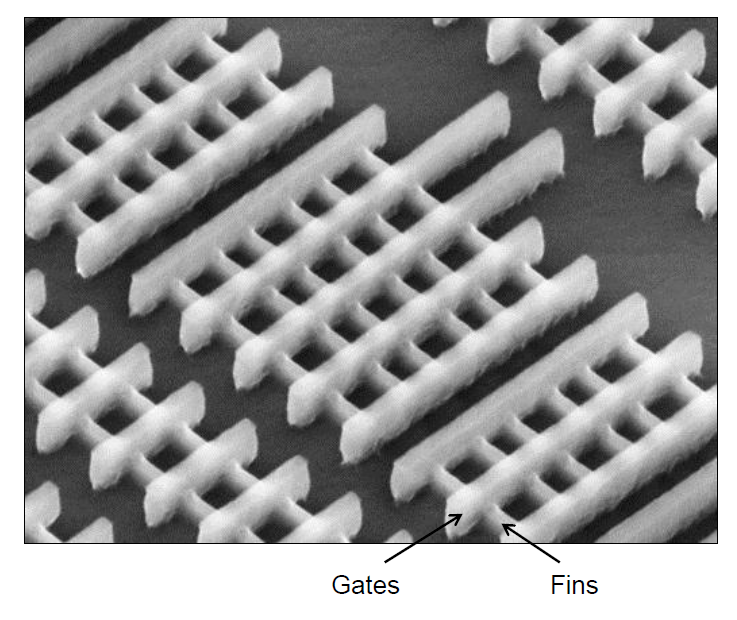
\includegraphics[width=0.7\textwidth]{intel-trigate}
 \end{center} 
 
\end{frame} 


\begin{frame} {Semiconductor Devices in 3D: FinFET} 
  
 \begin{center} 
   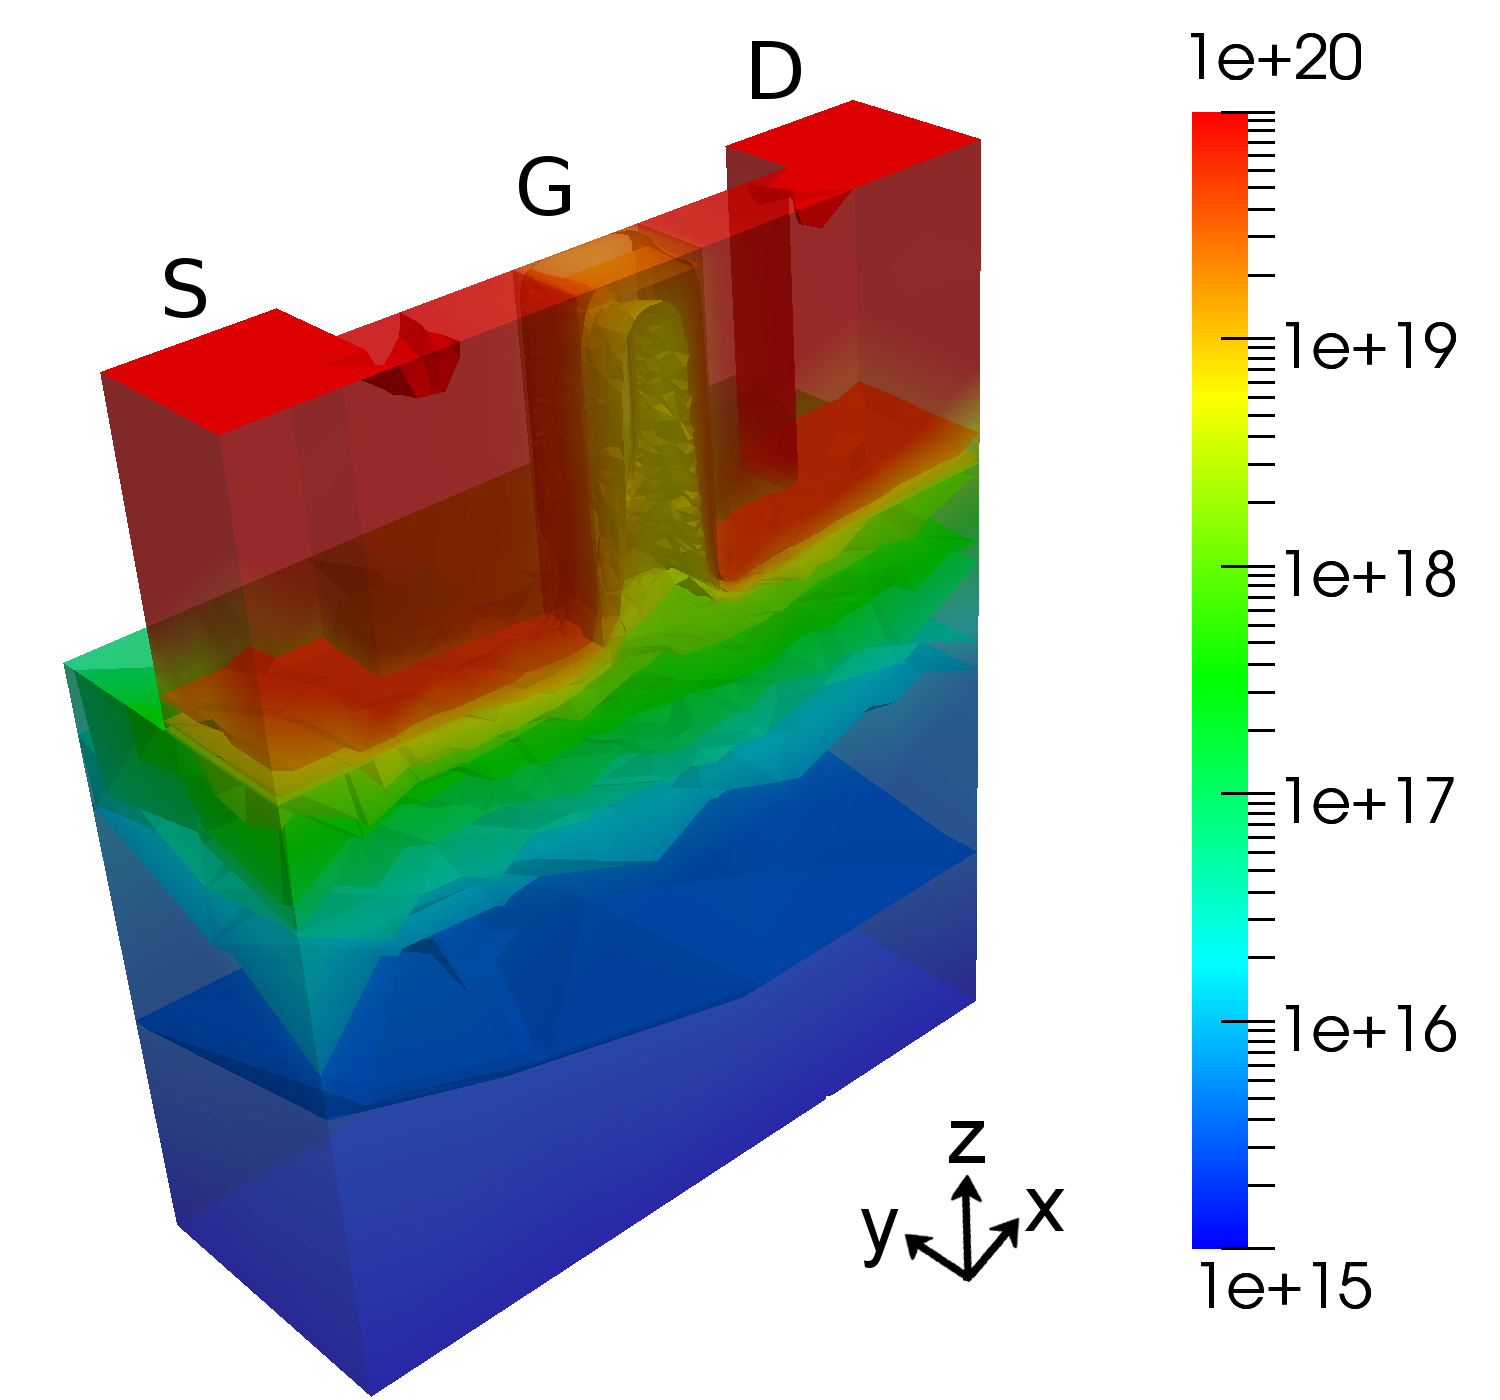
\includegraphics[width=0.6\textwidth]{trigate-n-2}
 \end{center} 
 
\end{frame} 


% \begin{frame} {Electron Density in a FinFET} 
%   
%  \begin{center} 
%   Density of electrons at each point $\vector x$ \\ 
%   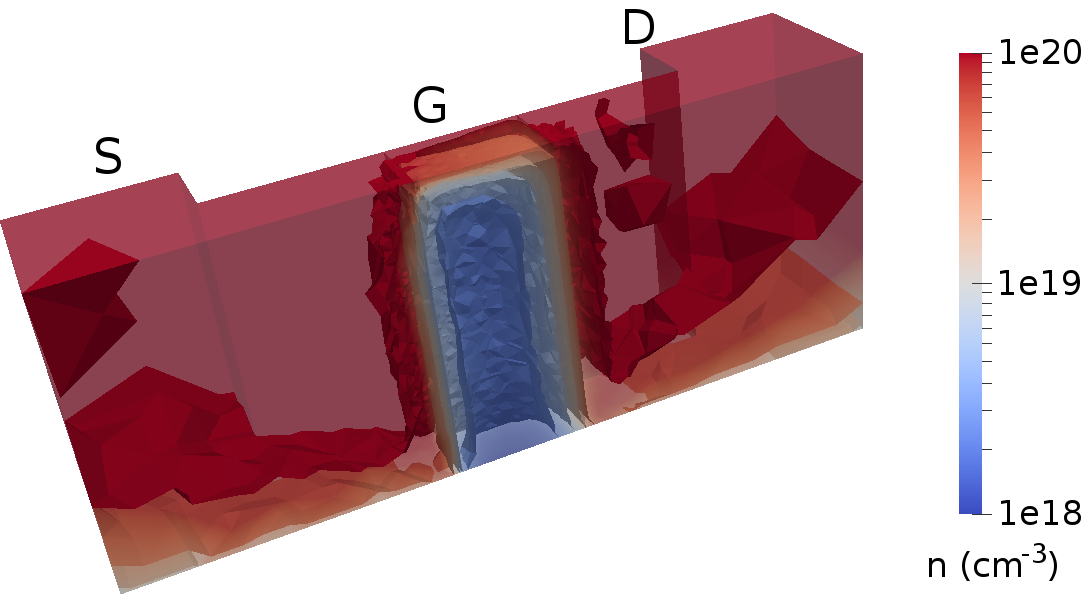
\includegraphics[width=0.632\textwidth]{trigate-electrons-mod}
%  \end{center} 
%   \vspace*{2.68cm}
%  
% \end{frame} 
%  
% 
% \begin{frame}{Electron Energy Distribution?} 
%  \begin{center} 
%   Distribution of electrons with respect to energy at $\vector x$? \\ 
%   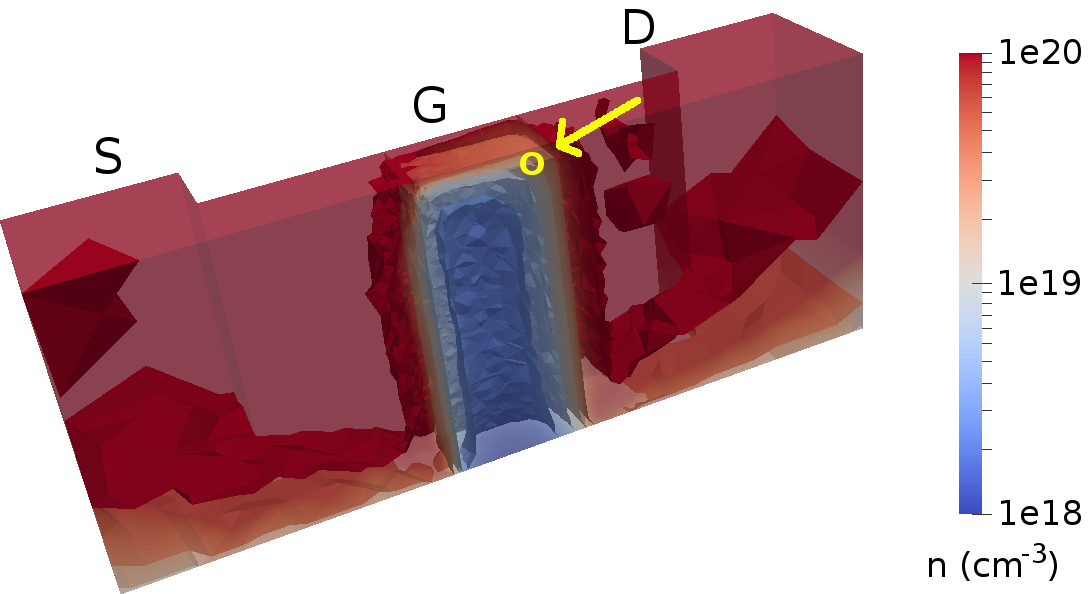
\includegraphics[width=0.632\textwidth]{trigate-electrons-mod2}
%  \end{center} 
%   \vspace*{2.68cm}
% \end{frame} 
%  
% \begin{frame} {Electron Energy Distribution?} 
%  \begin{center}Distribution of electrons with respect to energy at $\vector x$? \\ 
%   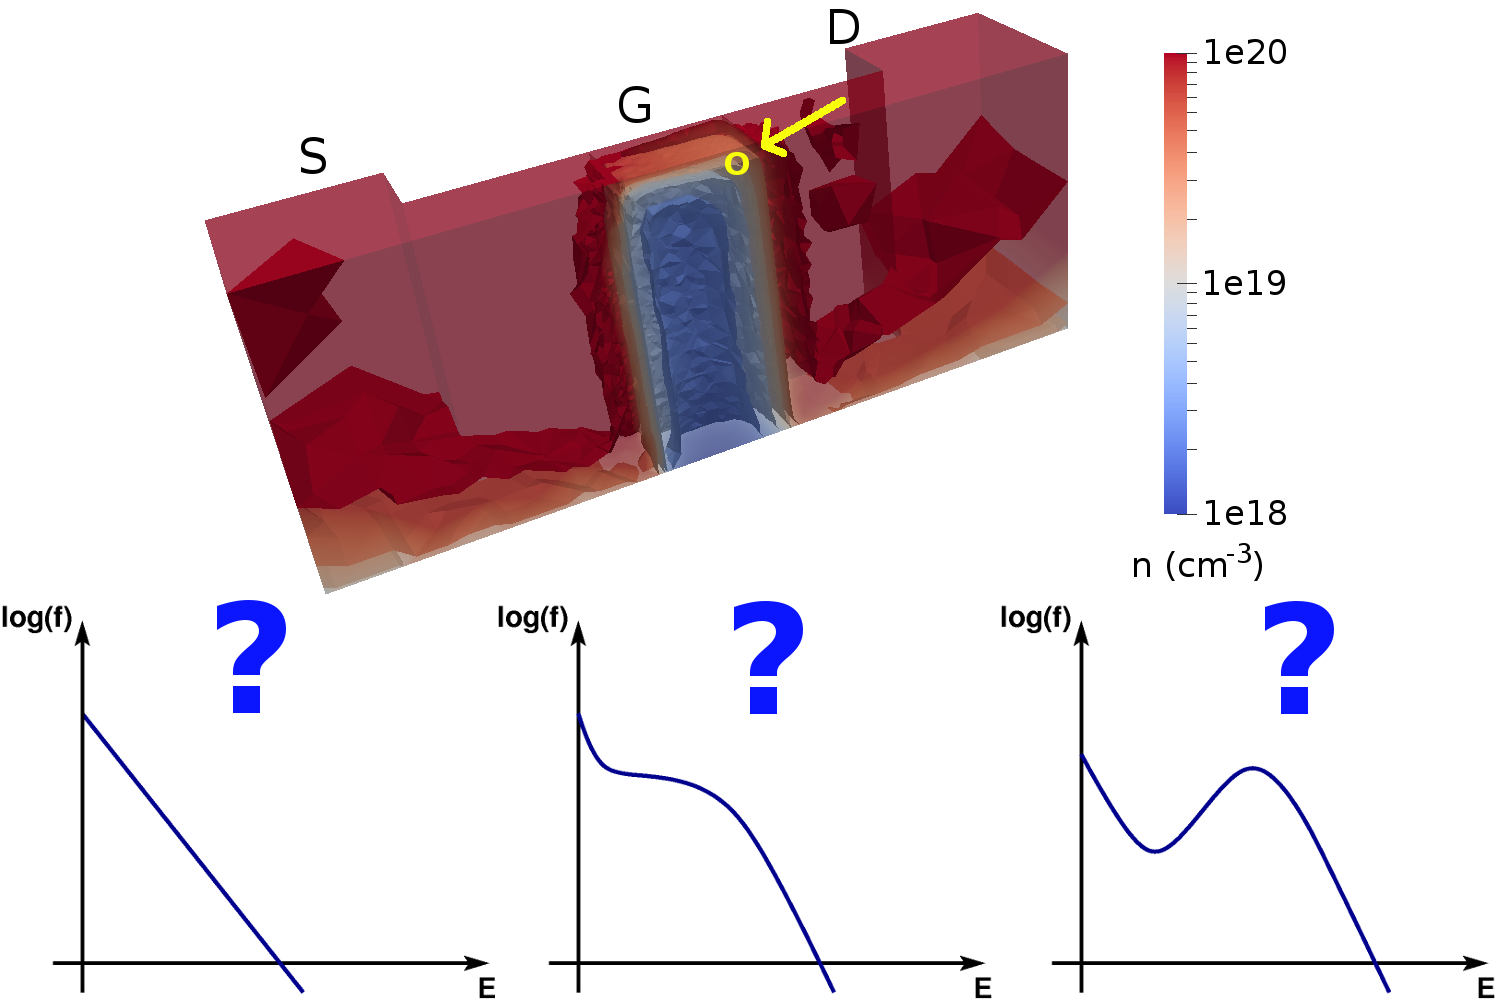
\includegraphics[width=0.87\textwidth]{trigate-electrons-edf-1}
%  \end{center} 
% \end{frame} 
%  
% \begin{frame} {Electron Energy Distribution?} 
%  \begin{center}Distribution of electrons with respect to energy at $\vector x$? \\ 
%   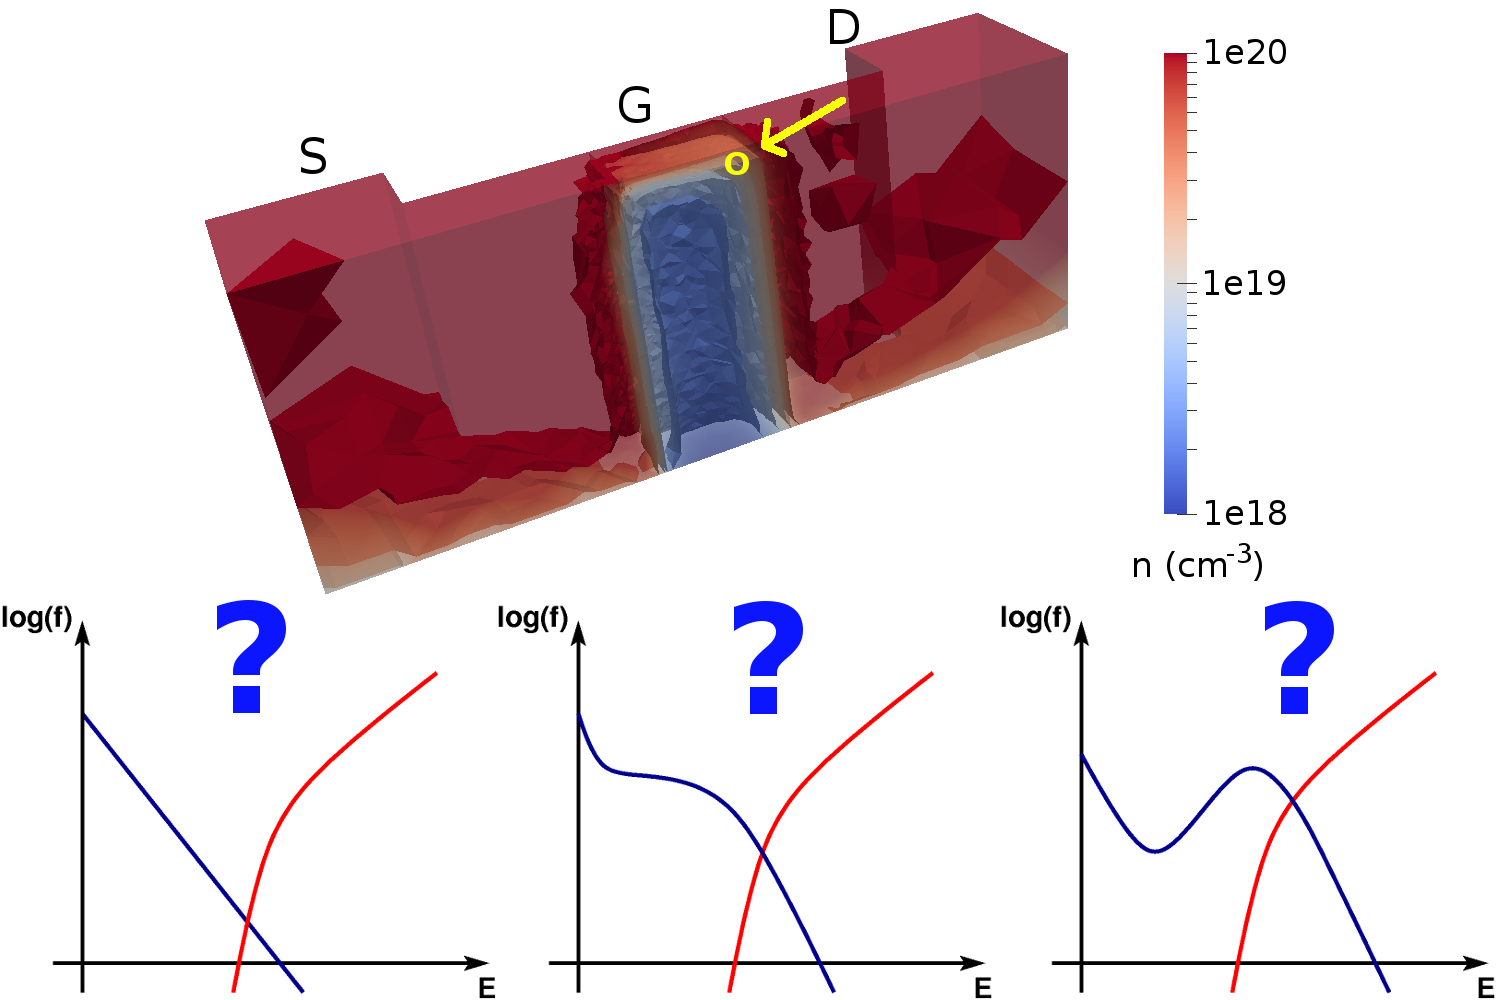
\includegraphics[width=0.87\textwidth]{trigate-electrons-edf-2}
%  \end{center} 
% \end{frame} 
 
\begin{frame} {Electron Energy Distribution?} 
 \begin{center}Distribution of electrons with respect to energy at $\vector x$? \\ 
  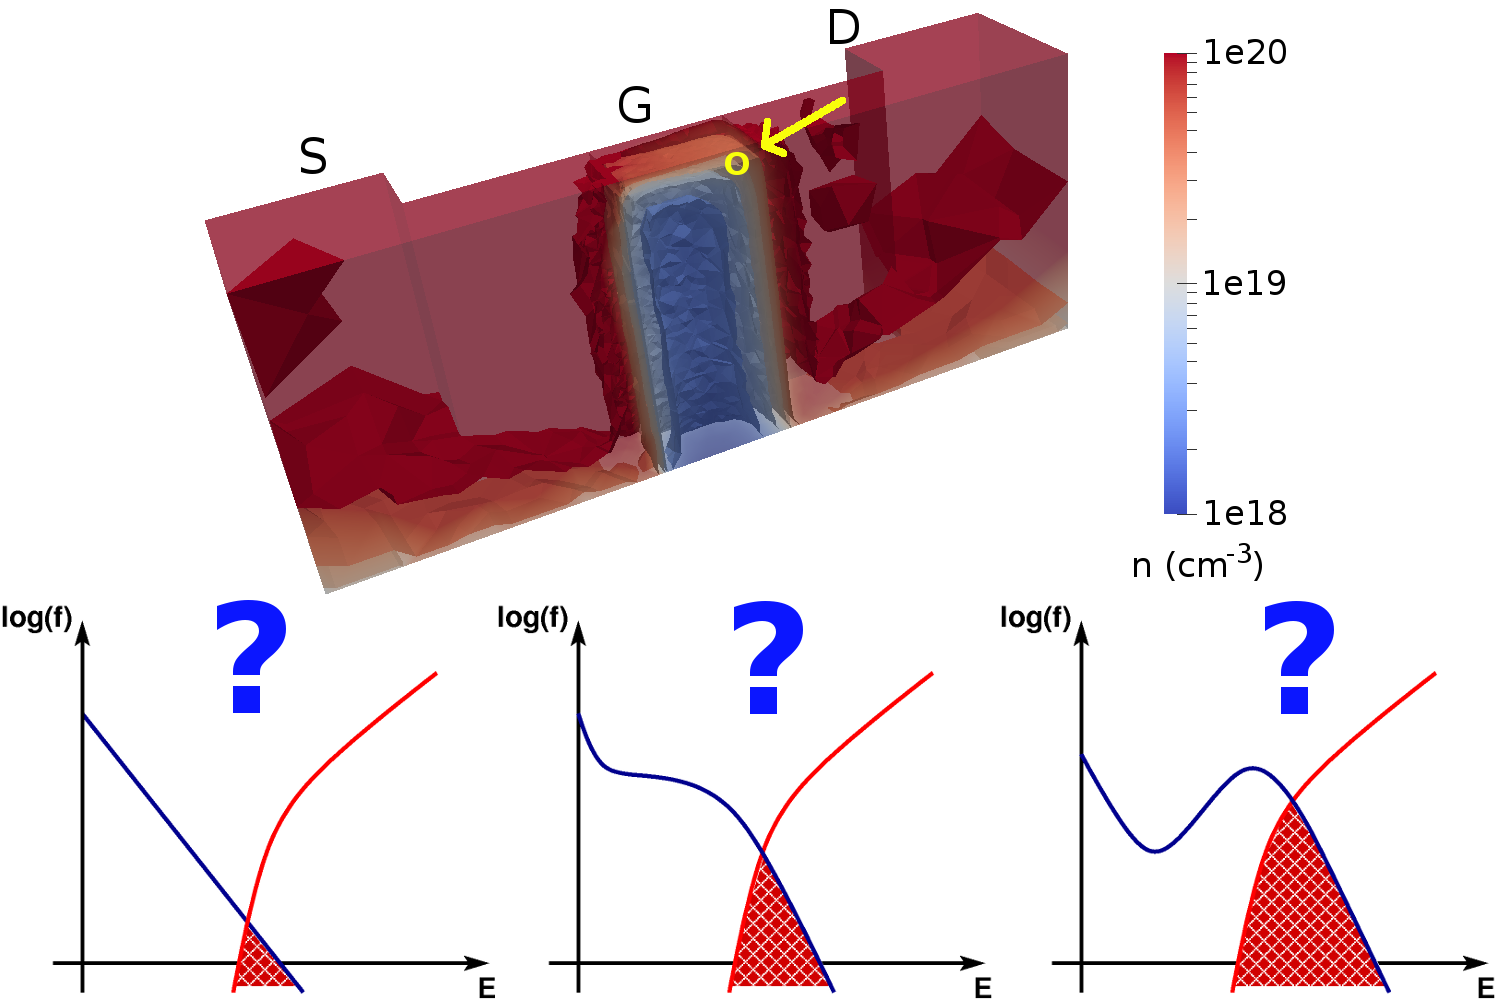
\includegraphics[width=0.87\textwidth]{trigate-electrons-edf-3}
 \end{center} 
\end{frame} 
 

\begin{frame} {Electron Energy Distribution?} 
 
  \begin{block}{Macroscopic Transport Models} 
    \begin{itemize} 
     \item Invalid in deca-nanometer regime 
     \item ``Fitting'' only treats the symptoms, not the cause 
     \item Only averaged quantities of the carrier ensemble modeled 
    \end{itemize} 
  \end{block} 
 
 %\visible<2->{
  \vspace*{0.5cm}
  \begin{block}{Boltzmann Transport Equation (BTE)} 
    \begin{align*} \Large 
      \frac{\partial f}{\partial t} +  \vector v(\vector k) \cdot \nabla_{\vector x} f + \vector F(\vector x) \cdot \nabla_{\vector k} f = Q\{f\}  
    \end{align*} 
  \vspace*{0.1cm}
 
    \begin{itemize} 
      \item Best semi-classical description of carrier transport 
      \item Posed in a seven-dimensional $(\vector x, \vector k, t)$ space 
      \item Most popular solution method: Monte Carlo 
    \end{itemize} 
  \end{block} 
  \vspace*{0.5cm}
 % }
\end{frame} 
 

% \begin{frame} {Electron Energy Distribution?}
%  \begin{center}
%   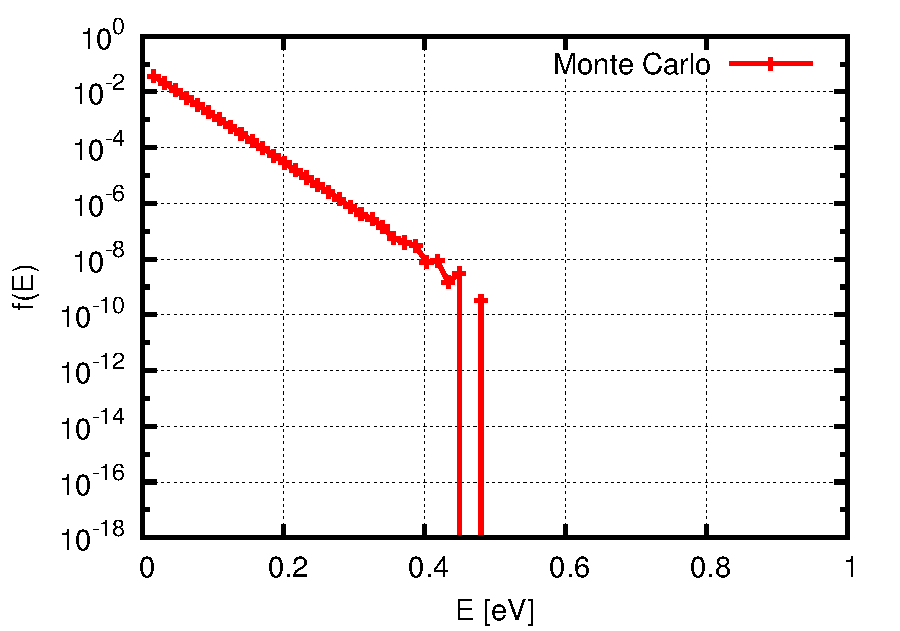
\includegraphics[width=0.95\textwidth]{she-monte-carlo-1}
%  \end{center}
% \end{frame}

\begin{frame} {Electron Energy Distribution?}
 \begin{center}
  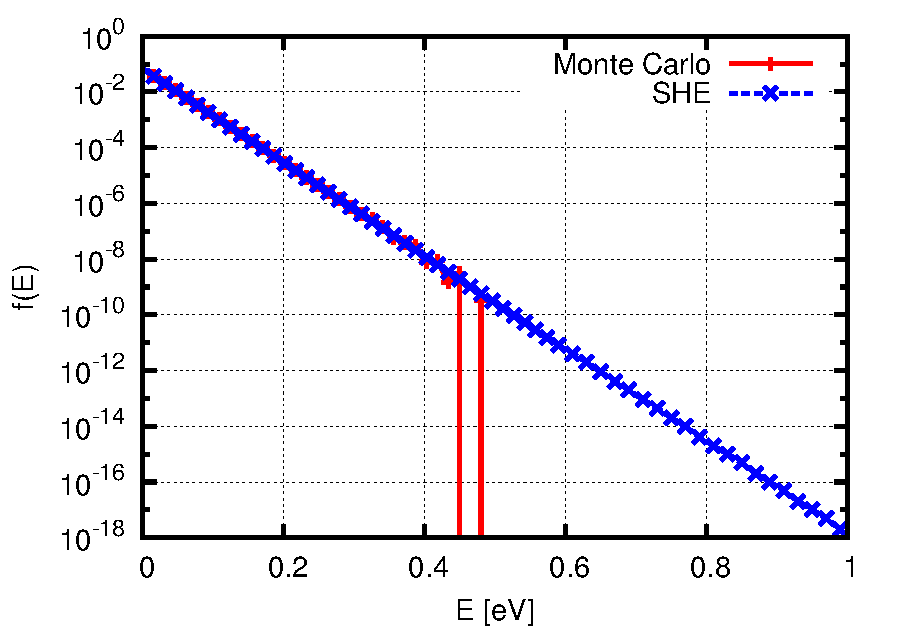
\includegraphics[width=0.95\textwidth]{she-monte-carlo-2}
 \end{center}
\end{frame}
 

\section{Spherical Harmonics Expansion Method}


% \begin{frame}{Spherical Harmonics Expansion Method}
% 
%  \vspace*{-0.3cm}
%   \begin{block}{Spherical Symmetries}
%   \begin{itemize}
%    \item Maxwell distribution of carriers at equilibrium
%    \item Dispersion relation (Herring-Vogt transform, approx.)
%   \end{itemize}
%   \end{block}
% 
%   \vspace*{-0.5cm}
%   \begin{block}{}
%    \begin{itemize}
%     \item 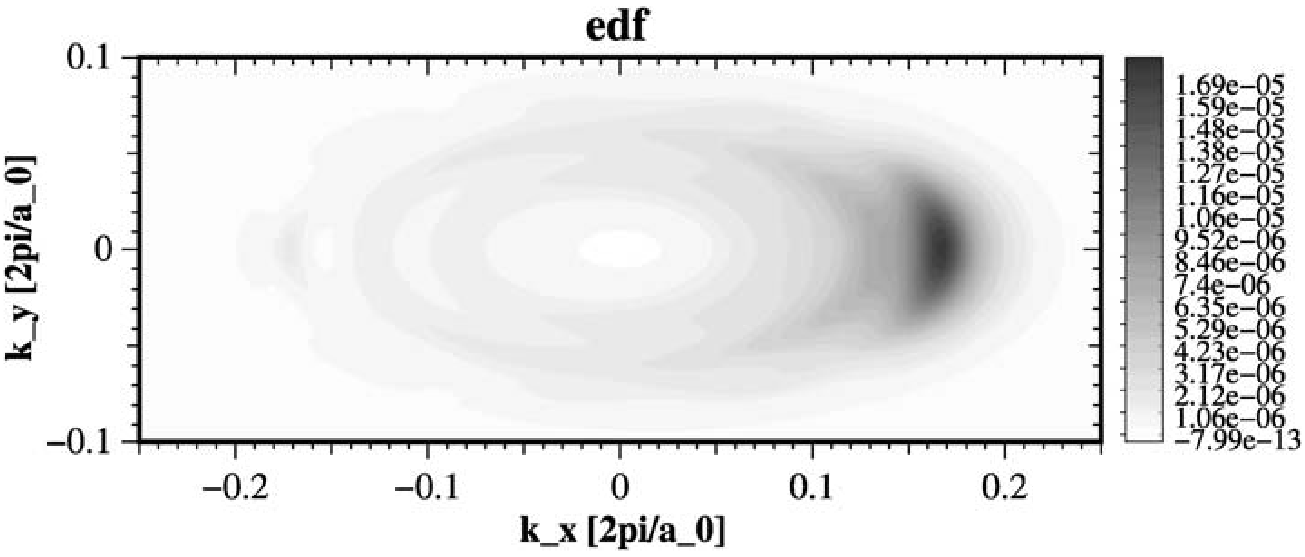
\includegraphics[width=0.78\textwidth]{edf}
%     \item {\scriptsize \ S.-M.~Hong and C.~Jungemann (2009)}
%    \end{itemize}
%   \end{block}
% 
% \end{frame}


\begin{frame}{Spherical Harmonics Expansion Method}

 \vspace*{-0.3cm}
  \begin{block}{Spherical Symmetries}
  \begin{itemize}
   \item Maxwell distribution of carriers at equilibrium
   \item Dispersion relation (Herring-Vogt transform, approx.)
  \end{itemize}
  \end{block}

 
     \vspace*{0.62cm}
  \begin{block}{Spherical Harmonics Expansion (SHE)}
     \vspace*{-0.5cm}
      { %\Large
       \begin{align*}
	f(\vector x, \vector k, t) \simeq \sum_{l = 0}^L \sum_{m=-l}^l f_{l,m}(\vector x, E, t) Y_{l,m}(\theta, \varphi)
      \end{align*}}
     \vspace*{-0.5cm}
    \begin{itemize}
     \item New unknowns: $f_{l,m}(\vector x, E, t)$
     \item Solution in five-dimensional $(\vector x, E, t)$-space
     \item S.-M.~Hong and C.~Jungemann, \textit{J Comput Electron} (2009): \\
           Fifth-order, three-dim.~$(\vector x, E)$-space, 26 GB memory, 12 hours
    \end{itemize}
   \end{block}
%     \vspace*{-0.4cm}


\end{frame}




% \begin{frame}{Spherical Harmonics Expansion Method}
% 
%  \vspace*{-0.68cm}
%   \begin{block}{}
%    \begin{itemize}
%     \item 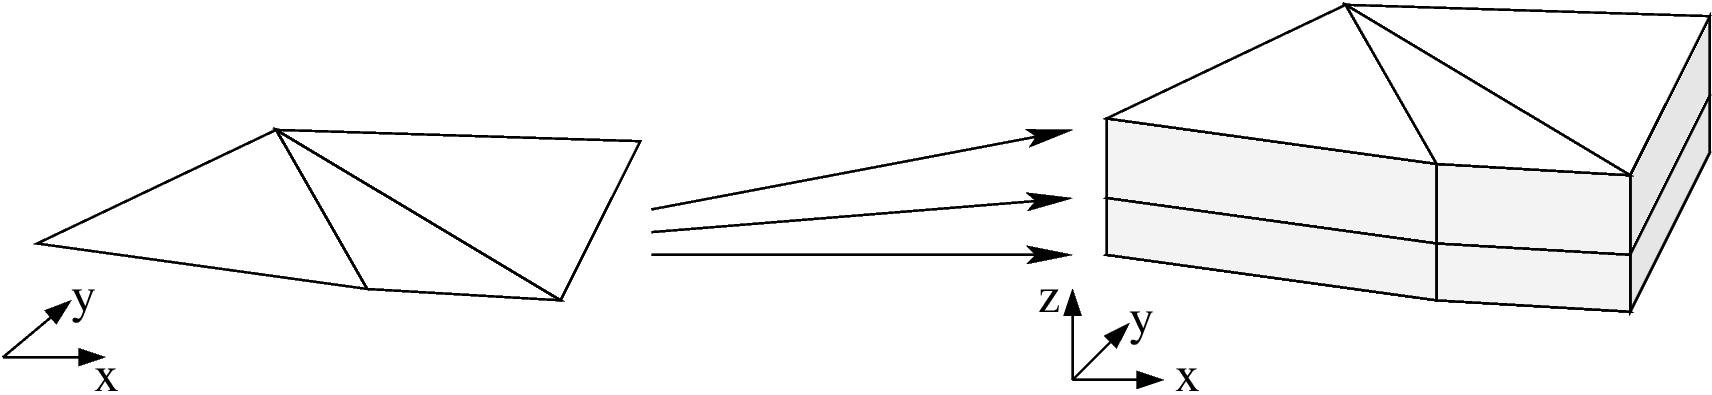
\includegraphics[width=0.8\textwidth]{prismatic}
%    \end{itemize}
%   \end{block}
% 
%   \begin{block}{Spherical Harmonics Expansion (SHE)}
%      \vspace*{-0.5cm}
%       { %\Large
%        \begin{align*}
% 	f(\vector x, \vector k, t) \simeq \sum_{l = 0}^L \sum_{m=-l}^l f_{l,m}(\vector x, E, t) Y_{l,m}(\theta, \varphi)
%       \end{align*}}
%      \vspace*{-0.5cm}
%     \begin{itemize}
%      \item New unknowns: $f_{l,m}(\vector x, E, t)$
%      \item Solution in five-dimensional $(\vector x, E, t)$-space
%      \item S.-M.~Hong and C.~Jungemann, \textit{J Comput Electron} (2009): \\
%            Fifth-order, three-dim.~$(\vector x, E)$-space, 26 GB memory, 12 hours
%     \end{itemize}
%    \end{block}
% 
% \end{frame}


%%
%%
%%  M E T H O D S
%%
%%


%
% Unstructured Grids
%


\section{Unstructured Grids}

\begin{frame}{Unstructured Grids}
%  \vspace*{-0.5cm}
 \begin{block}{Unstructured Grids}
  \begin{itemize}
   \item State-of-the-art in modern TCAD
   \item Only structured grids in publications on higher-order SHE in 2D  \\
         \hspace{0.3cm} {\footnotesize [S.-M.~Hong and C.~Jungemann (2008), S.-M.~Hong and C.~Jungemann (2009)] }
   \item Extension of discretization proposed by Hong and Jungemann
  \end{itemize}
 \end{block}

 \begin{center}
  \begin{minipage}{0.2\textwidth}
    4838 nodes
  \end{minipage}
  \begin{minipage}{0.55\textwidth}
    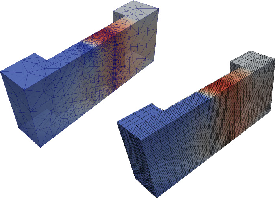
\includegraphics[width=0.95\textwidth]{tetsortho}\ \ \\
  \end{minipage}
  \begin{minipage}{0.2\textwidth}
    27456 nodes
  \end{minipage}
 \end{center}
\end{frame}



% \begin{frame}{Summary}
%   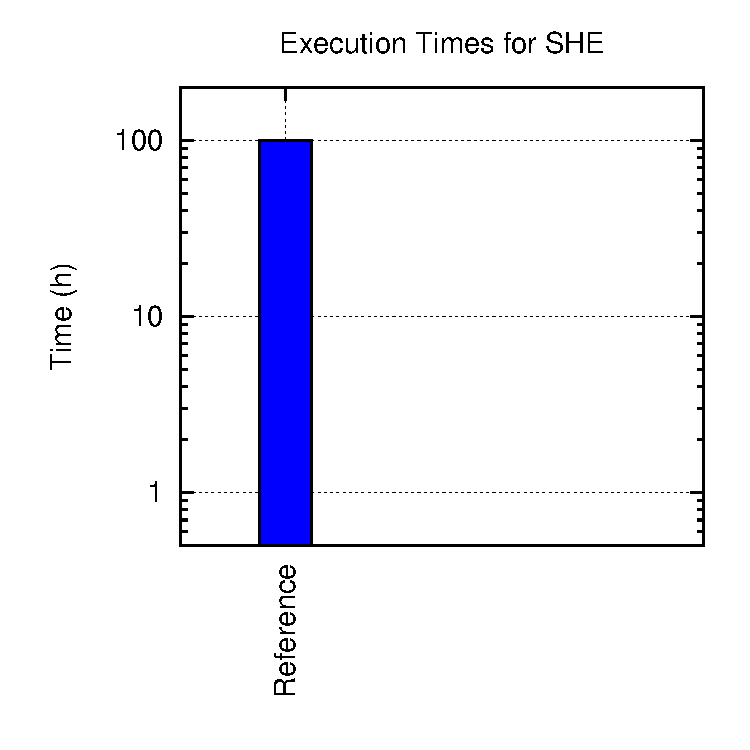
\includegraphics[width=0.49\textwidth]{summary-exec-1}
%   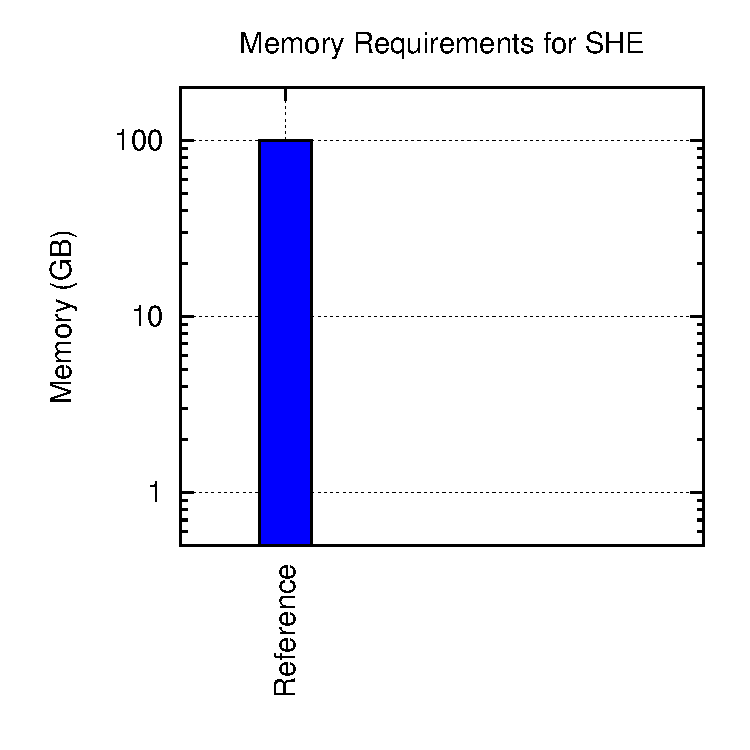
\includegraphics[width=0.49\textwidth]{summary-memory-1}
% \end{frame}

\begin{frame}{Summary}
 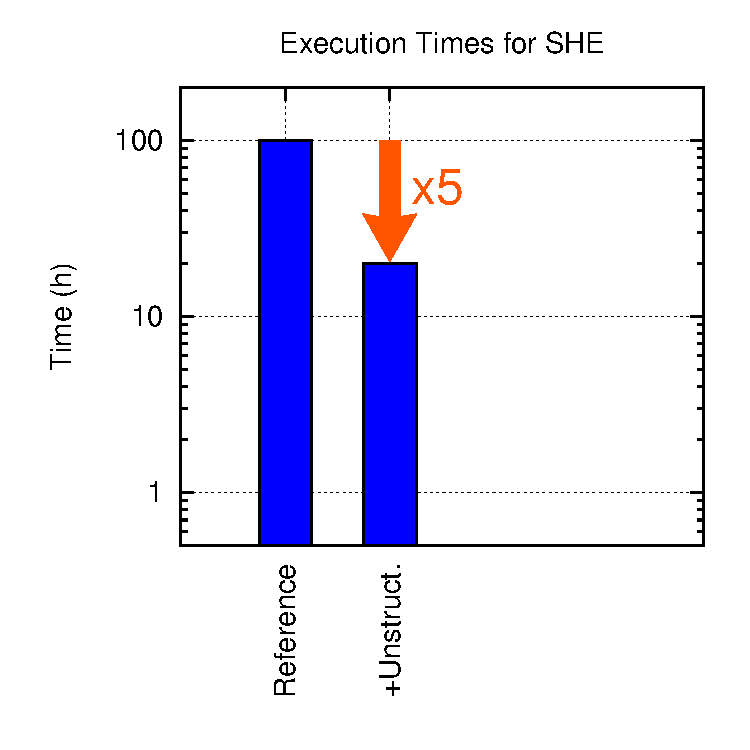
\includegraphics[width=0.49\textwidth]{summary-exec-2}
 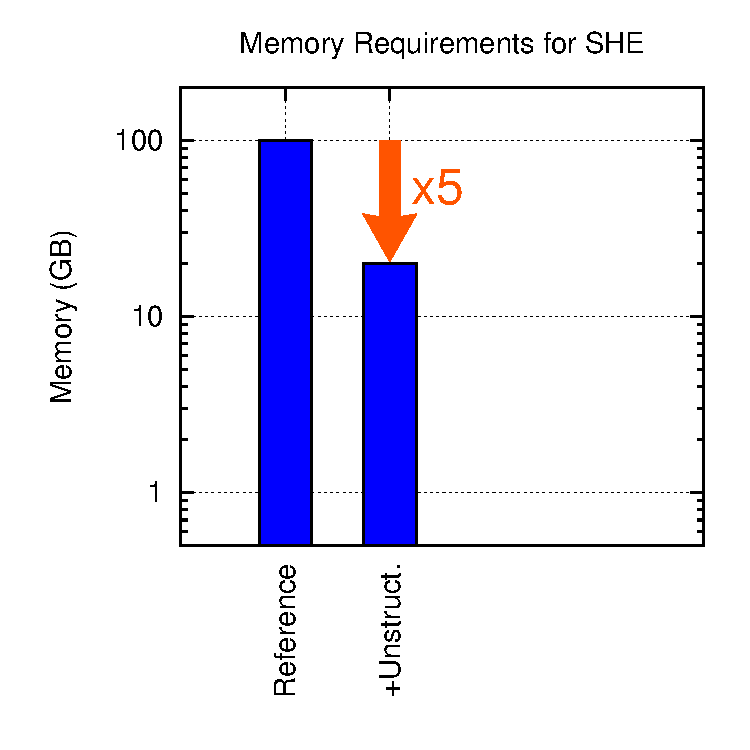
\includegraphics[width=0.49\textwidth]{summary-memory-2}
\end{frame}




%
% Adaptive Variable-Order
%

\section{Adaptive Variable-Order SHE}

% \begin{frame}{Adaptive Variable-Order SHE}
%   \vspace*{-0.05cm}
%   \begin{block}{Spherical Harmonics Expansion}
%      \vspace*{-0.6cm}
%       { \begin{align*}
% 	f(\vector x, \vector k, t) \simeq \sum_{l = 0}^L \sum_{m=-l}^l f_{l,m}(\vector x, E, t) Y_{l,m}(\theta, \varphi)
%       \end{align*}}
%      \vspace*{-0.6cm}
%   \end{block}
% 
%   \begin{itemize}
%    \item $(L+1)^2$ unknown functions $f_{l,m}(\vector x, E, t)$
%    \item $L=0$ sufficient in equilibrium
%    \item Higher-order expansions in active regions
%          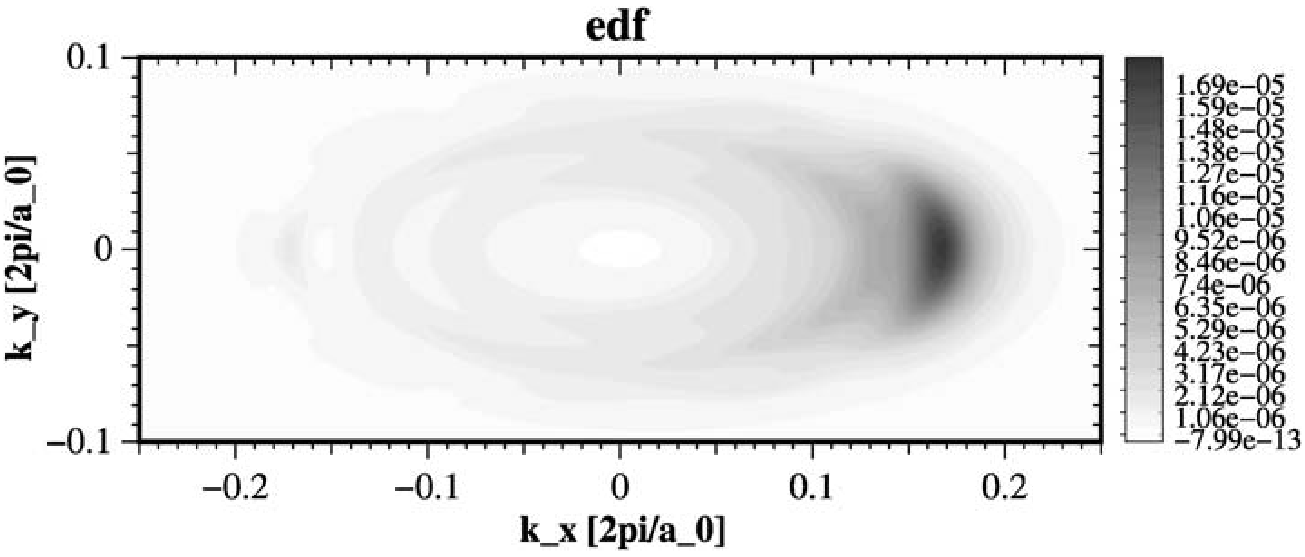
\includegraphics[width=0.78\textwidth]{edf}
%    \item {\scriptsize \ S.-M.~Hong and C.~Jungemann (2009)}
%   \end{itemize}
% %     \vspace*{-0.7cm}
% \end{frame}
% 


\begin{frame}{Adaptive Variable-Order SHE}

  \vspace*{-0.05cm}
  \begin{block}{Spherical Harmonics Expansion}
     \vspace*{-0.6cm}
      { \begin{align*}
	f(\vector x, \vector k, t) \simeq \sum_{l = 0}^L \sum_{m=-l}^l f_{l,m}(\vector x, E, t) Y_{l,m}(\theta, \varphi)
      \end{align*}}
     \vspace*{-0.6cm}
  \end{block}

  \begin{itemize}
   \item $(L+1)^2$ unknown functions $f_{l,m}(\vector x, E, t)$
   \item $L=0$ sufficient in equilibrium
   \item Higher-order expansions in active regions
   \item Therefore: Variable-order SHE:
      { \Large \begin{align*}
	f(\vector x_i, \vector k_n, t) \simeq \sum_{l = 0}^{L(\vector x_i, E_n)} \sum_{m=-l}^l f_{l,m}(\vector x_i, E_n, t) Y_{l,m}(\theta, \varphi)
      \end{align*}}
   \item How to choose $L(\vector x_i, E_n)$ in the simulation domain?
  \end{itemize}
     \vspace*{0.92cm}
\end{frame}





\begin{frame}{Adaptive Variable-Order SHE}
  
 \begin{block}{Motivation from Fourier series}

  \vspace*{0.6cm}
  \begin{minipage}{0.97\textwidth}
    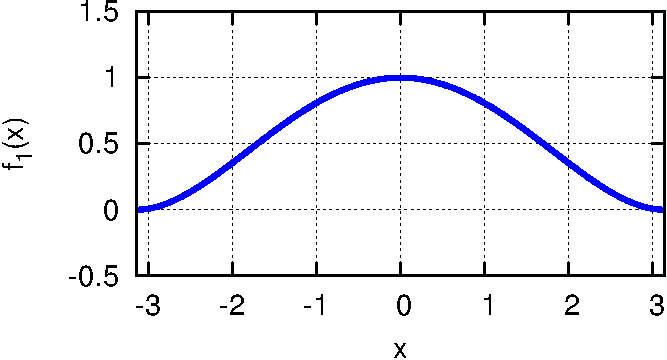
\includegraphics[width=0.45\textwidth]{fourier_f1} \hspace*{0.25cm}
    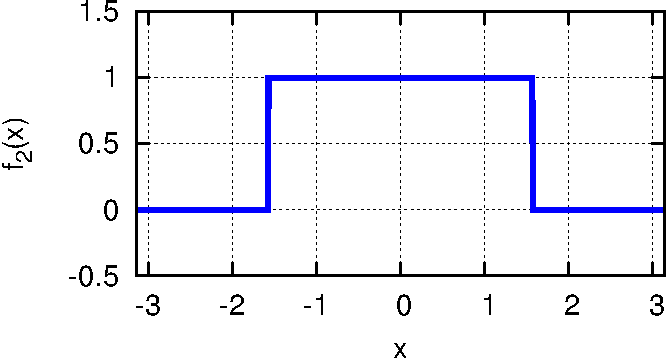
\includegraphics[width=0.45\textwidth]{fourier_f2} \hspace*{0.25cm} \newline

    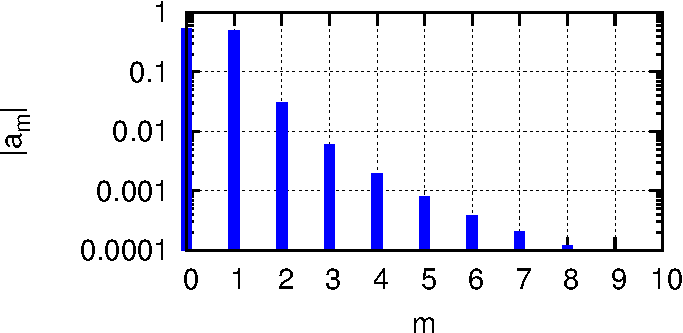
\includegraphics[width=0.45\textwidth]{fourier_coeff_1}\hspace*{0.25cm}
    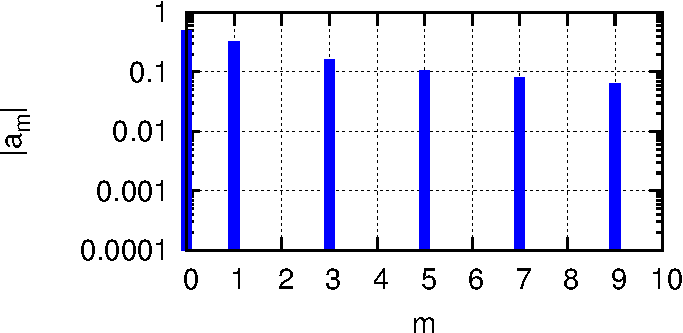
\includegraphics[width=0.45\textwidth]{fourier_coeff_2}
  \end{minipage}
 \end{block}

\end{frame}




\begin{frame}{Adaptive Variable-Order SHE}

 \fcolorbox{white}{white}{
  \begin{minipage}{0.1\textwidth}
    $L=1$ \\ 
    \vspace*{3cm} \\
    $L=3$
  \end{minipage}


  \begin{minipage}{0.4\textwidth}
  \begin{center} Error indicator:\\
    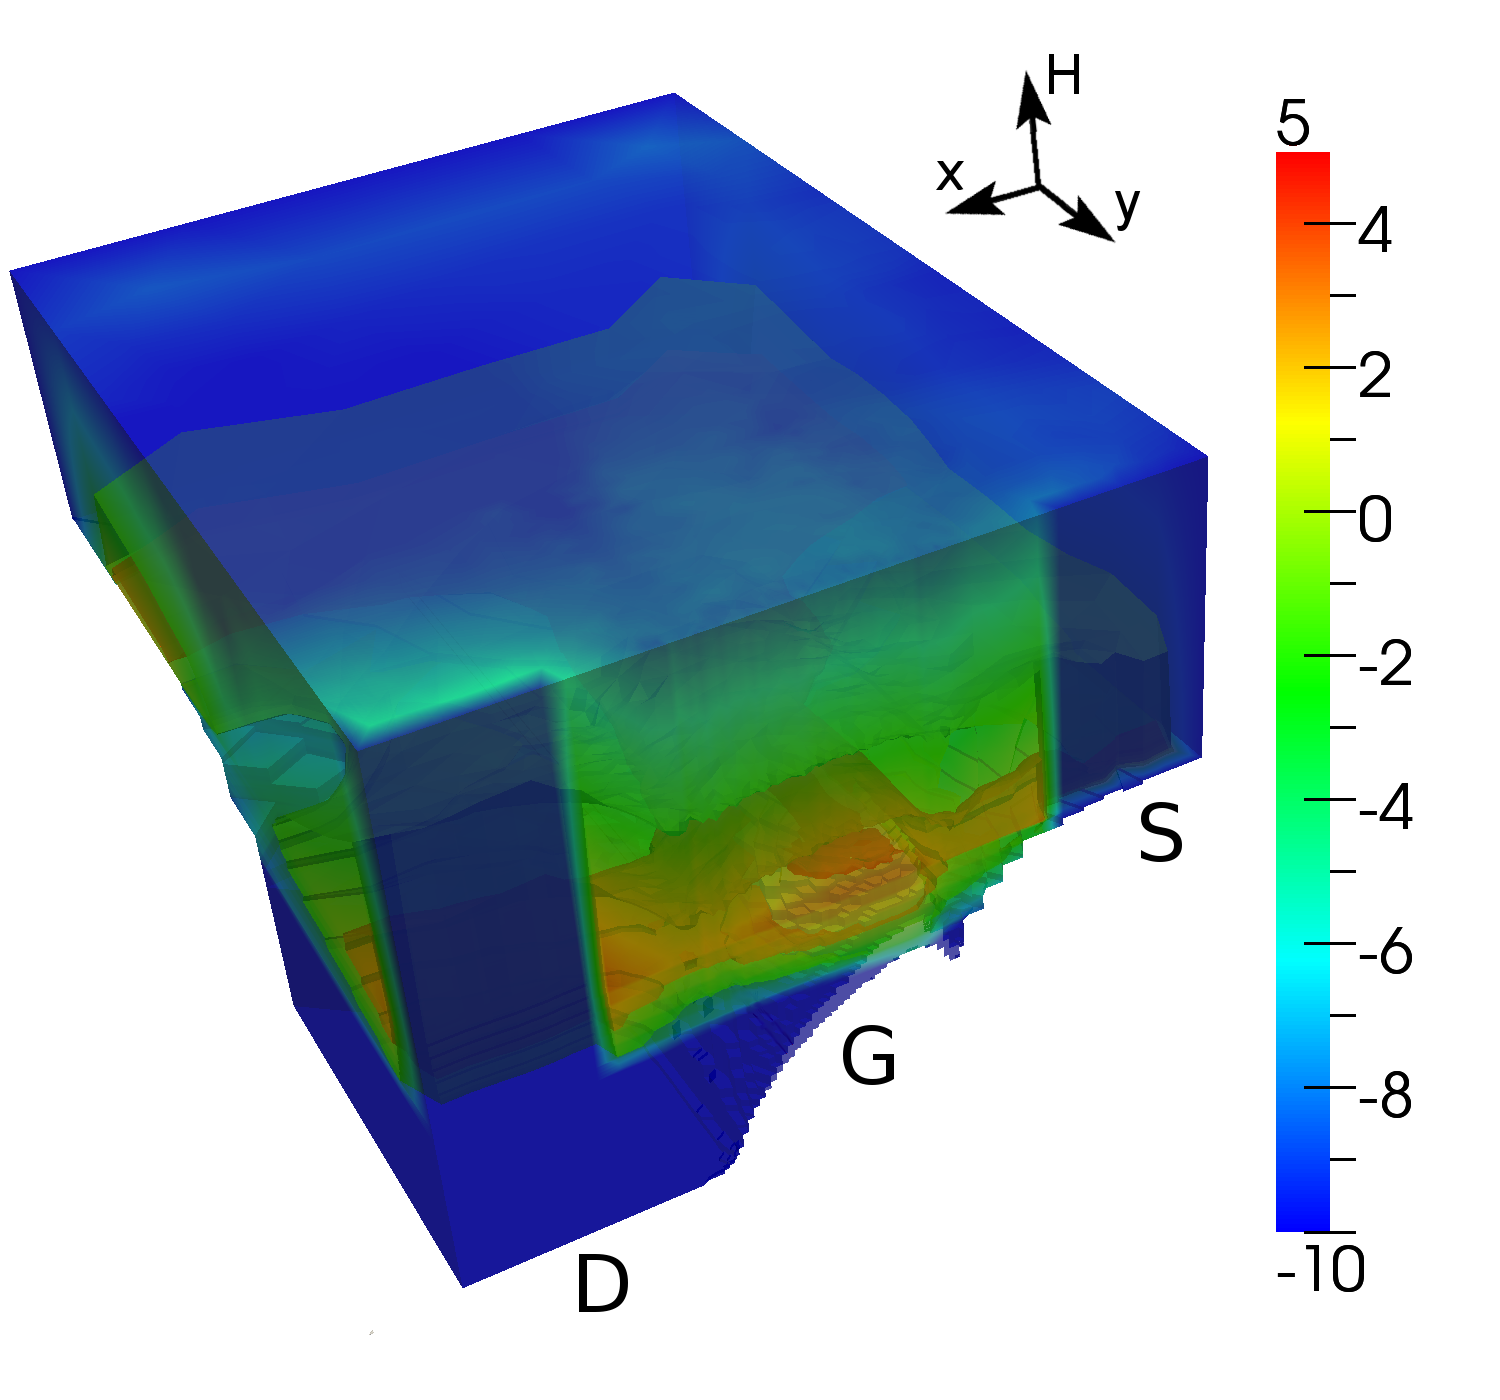
\includegraphics[width=0.9\textwidth]{mosfet-indicator-1} \\
    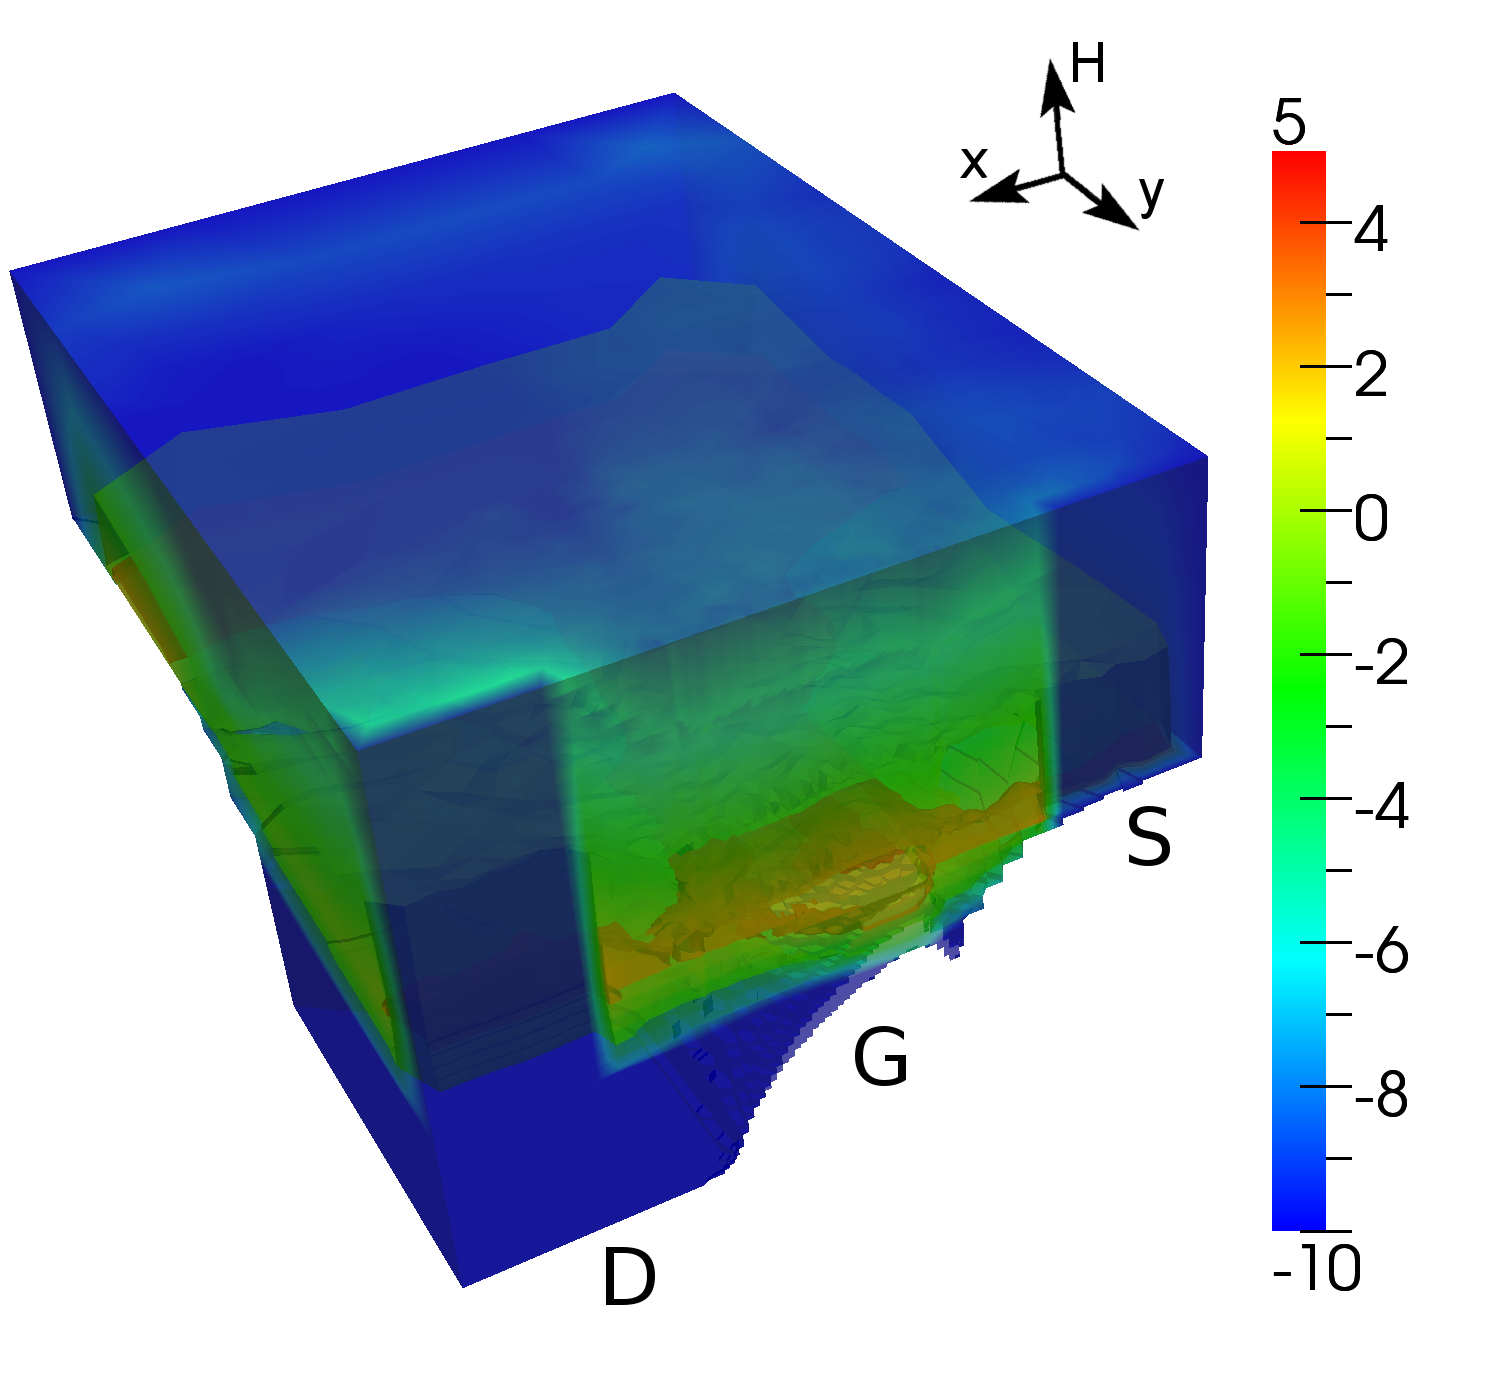
\includegraphics[width=0.9\textwidth]{mosfet-indicator-3}
  \end{center}
  \end{minipage}
  \hspace{0.5cm}
  \begin{minipage}{0.4\textwidth}
  \begin{center} Expansion order:\\
    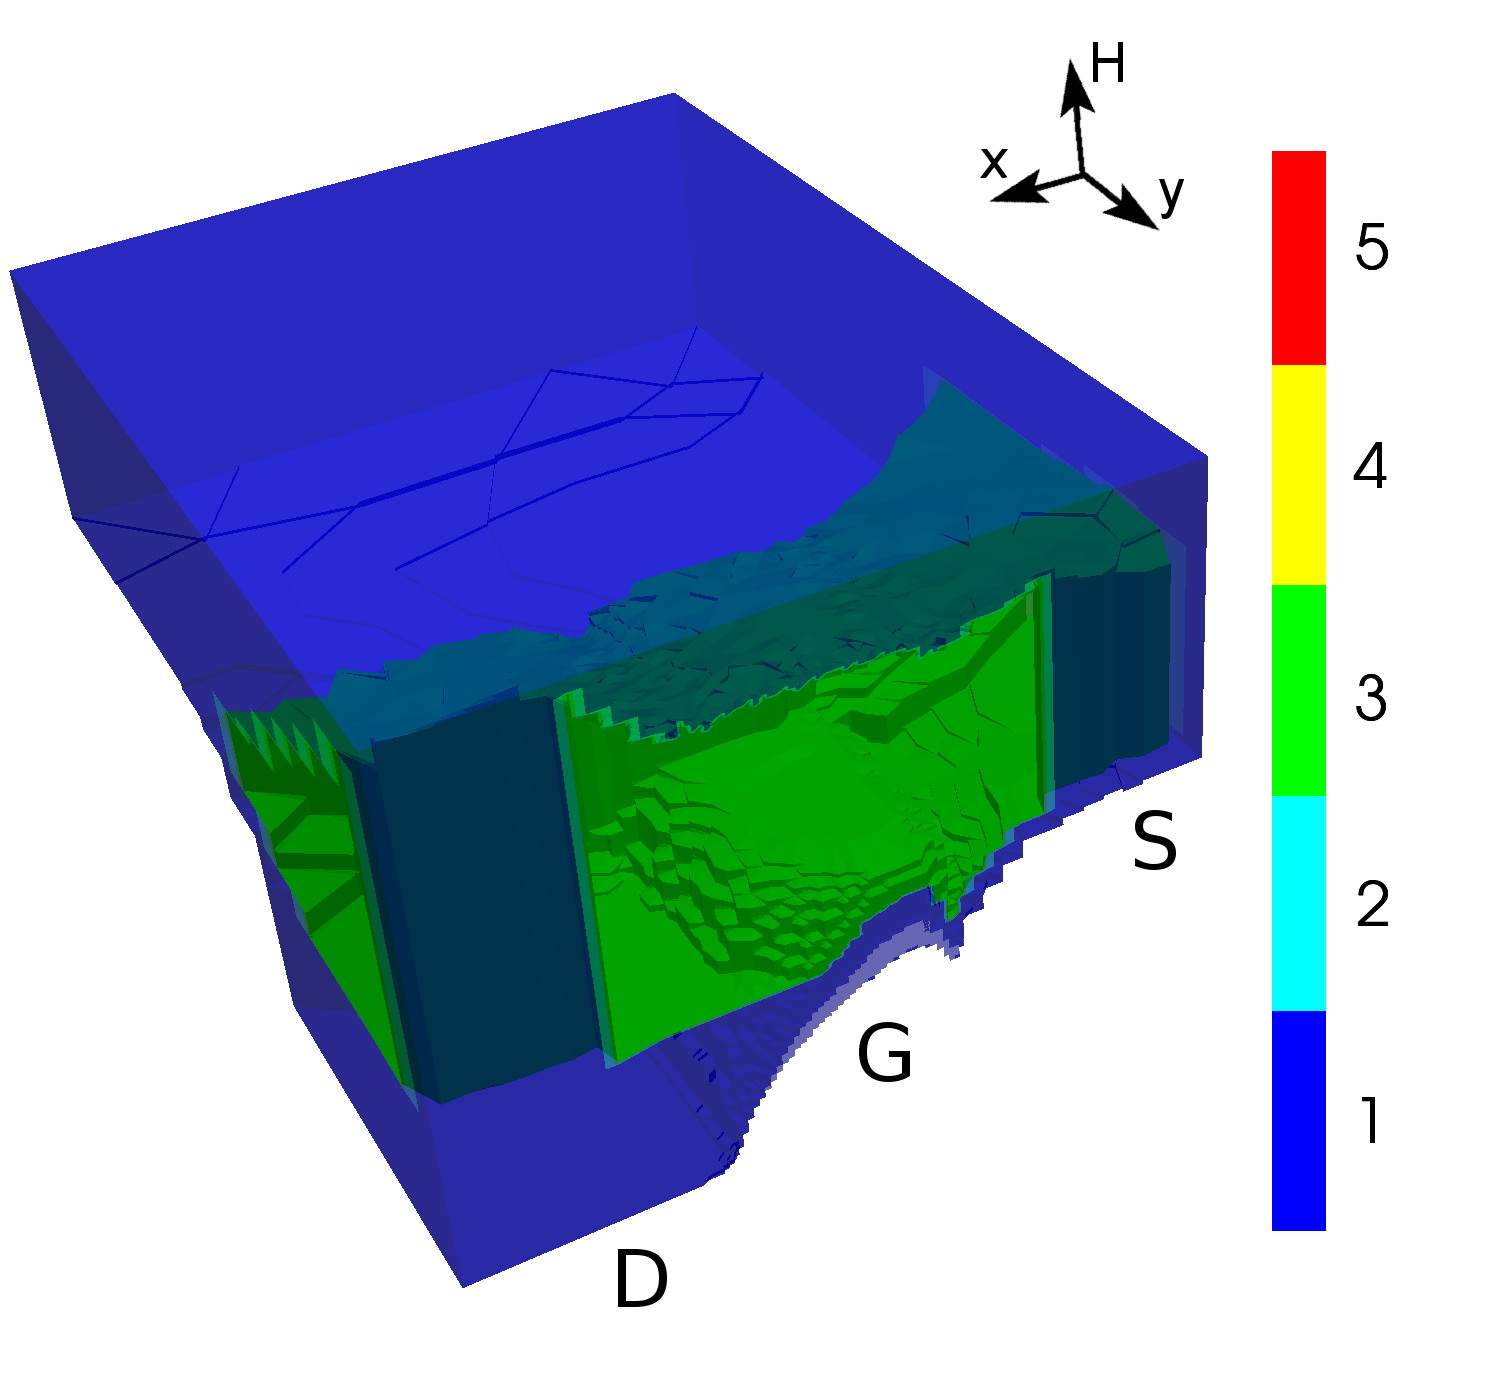
\includegraphics[width=0.9\textwidth]{mosfet-order-1} \\
    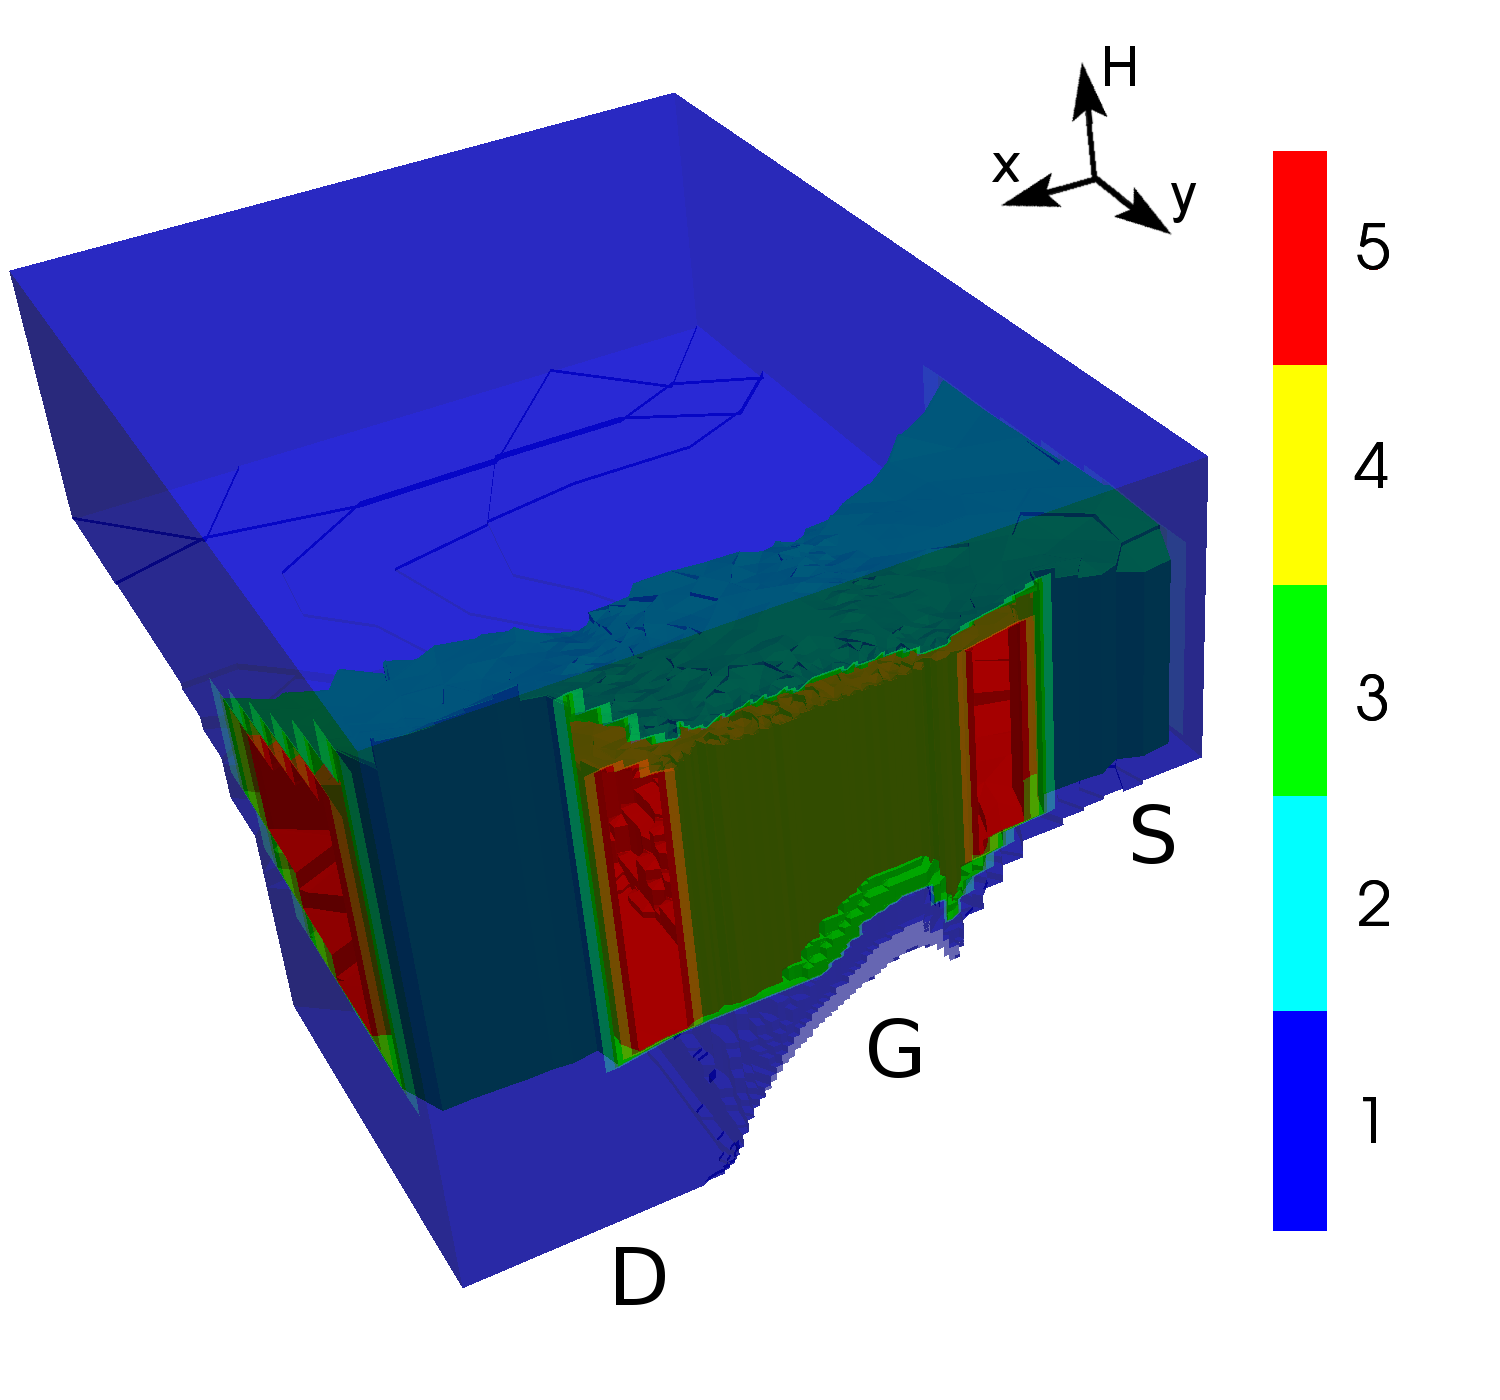
\includegraphics[width=0.9\textwidth]{mosfet-order-3}
    %\vspace*{1cm}
  \end{center}  
  \end{minipage}
  \hspace{2.5cm}
 } %end of fcolorbox

%   \vspace*{-0.5cm}
\end{frame}


\begin{frame}{Adaptive Variable-Order SHE}
  \vspace{-0.3cm}
  \begin{center}
   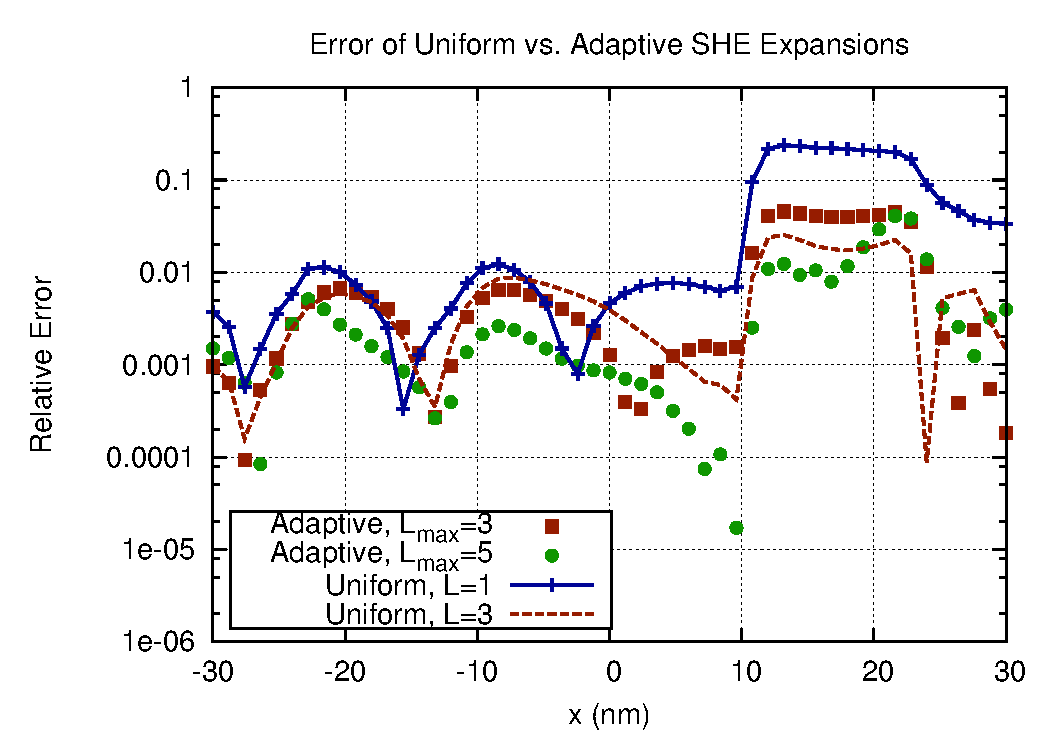
\includegraphics[width=0.75\textwidth]{mosfet-energy-error}
  \end{center}
  \vspace{-0.4cm}
  \begin{center}
   %\begin{itemize}
    %\item 
      $L=3$: $\mathbf{306\, 261}$ instead of $\mathbf{\hphantom{1}\, 476\, 061}$ unknowns (factor $\mathbf{1.5}$) \\
    %\item 
      $L=5$: $\mathbf{606\, 671}$ instead of $\mathbf{1\, 146\, 120}$ unknowns (factor $\mathbf{1.9}$)
   %\end{itemize}
  \end{center}
%   \vspace*{-0.5cm}
   
\end{frame}

% \begin{frame}{Summary}
%  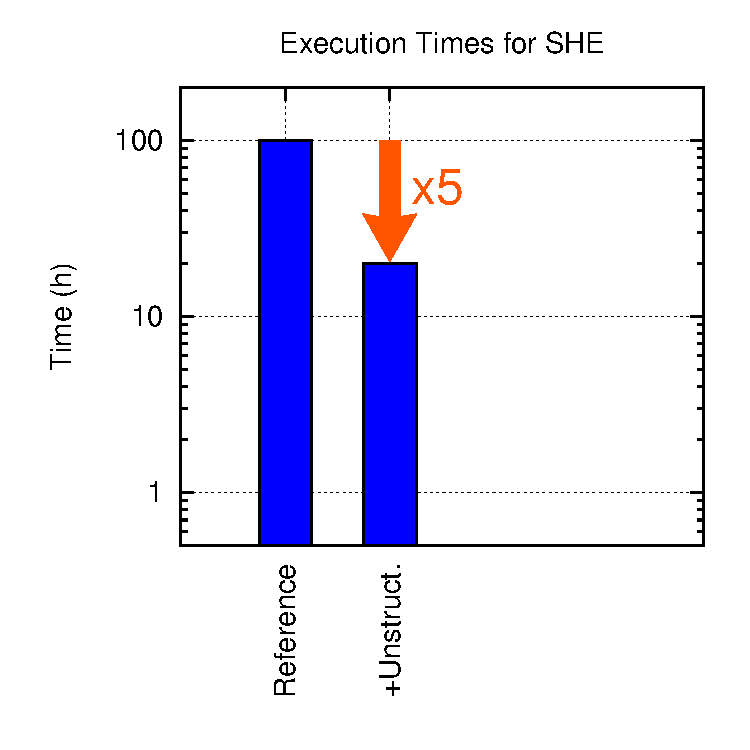
\includegraphics[width=0.49\textwidth]{summary-exec-2}
%  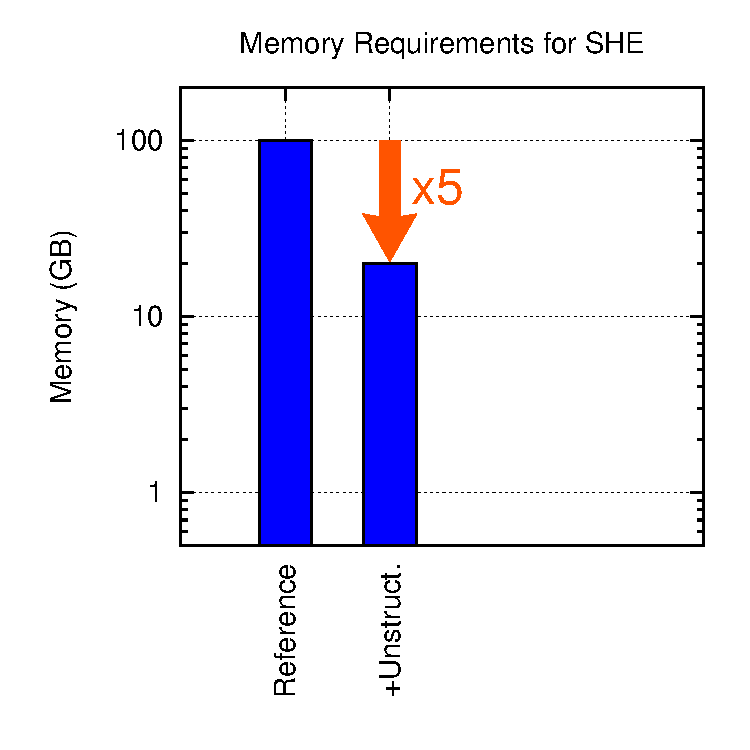
\includegraphics[width=0.49\textwidth]{summary-memory-2}
% \end{frame}

\begin{frame}{Summary}
  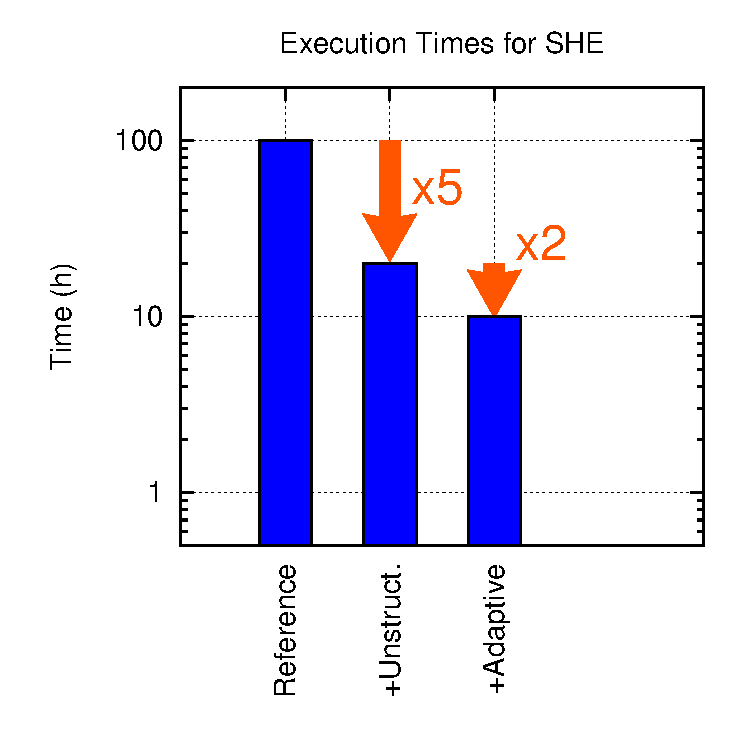
\includegraphics[width=0.49\textwidth]{summary-exec-3}
  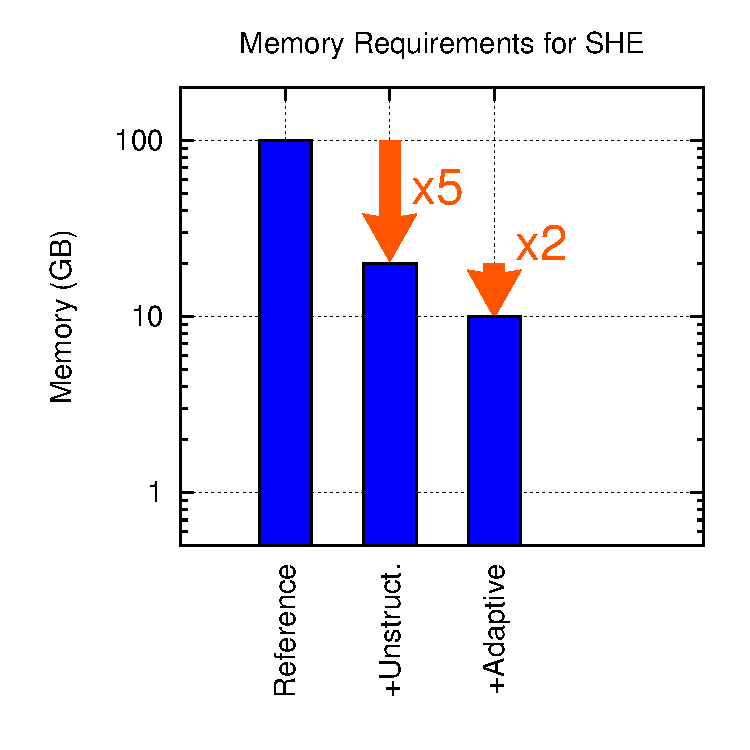
\includegraphics[width=0.49\textwidth]{summary-memory-3}
\end{frame}


%
% Parallelization
%

\section{Parallelization}

% \begin{frame}{Parallelization}
%  \begin{block}{Preconditioner for Iterative Linear Solvers}
%   \begin{itemize}
%    \item No fast general-purpose parallel preconditioner available
%    \item Physics-based parallel block preconditioner developed
%   \end{itemize}
%   \begin{center}
%    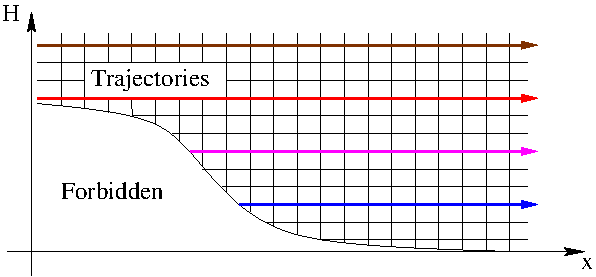
\includegraphics[width=0.8\textwidth]{electron-trajectory}
%   \end{center}
%  \end{block}
% %  \vspace*{-0.4cm}
% 
% \end{frame}

\begin{frame}{Parallelization}
 \begin{block}{Preconditioner for Iterative Linear Solvers}
  \begin{itemize}
   \item No fast general-purpose parallel preconditioner available
   \item Physics-based parallel block preconditioner developed
  \end{itemize}
  \begin{center}
   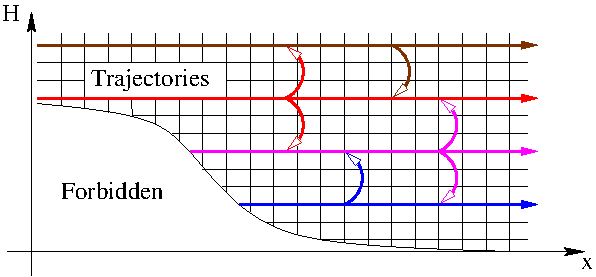
\includegraphics[width=0.8\textwidth]{electron-trajectory-2}
  \end{center}
 \end{block}
%  \vspace*{-0.4cm}

\end{frame}


\begin{frame}{Parallelization}
 \begin{block}{Scaling of Solution Variables}
  \begin{itemize}
   \item Exponential decay with energy: $f(E_i) \sim \exp(- \frac{E_i}{k_\mathrm{B} T})$
   \item Rescale unknowns: $\tilde{f}(E_i) = \exp( \frac{E_i}{k_\mathrm{B} T}) f(E_i)$
   %\item New system: $\tilde{\matrix A} \tilde{\vector x} = \matrix A \matrix D \matrix D^{-1} \vector x = \vector b$
   %\item Row normalization: $\hat{\matrix A} \tilde{\vector x} = \matrix P \tilde{\matrix A} \tilde{\vector x} = \matrix P \vector b$
  \end{itemize}
  \begin{center}
   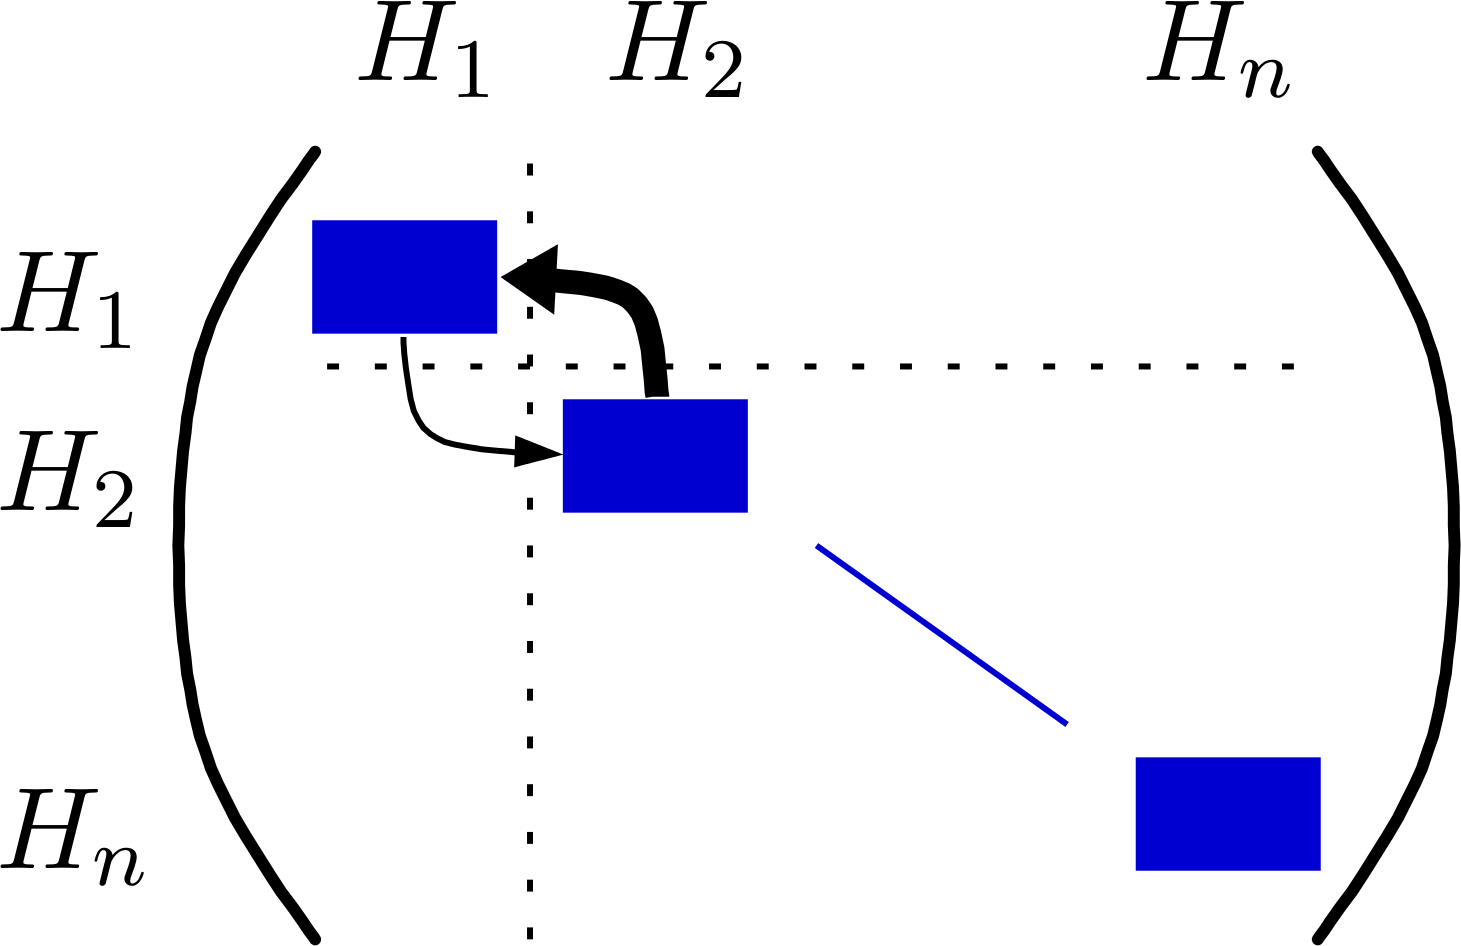
\includegraphics[width=0.45\textwidth]{matrix-structure-1} \hfill
   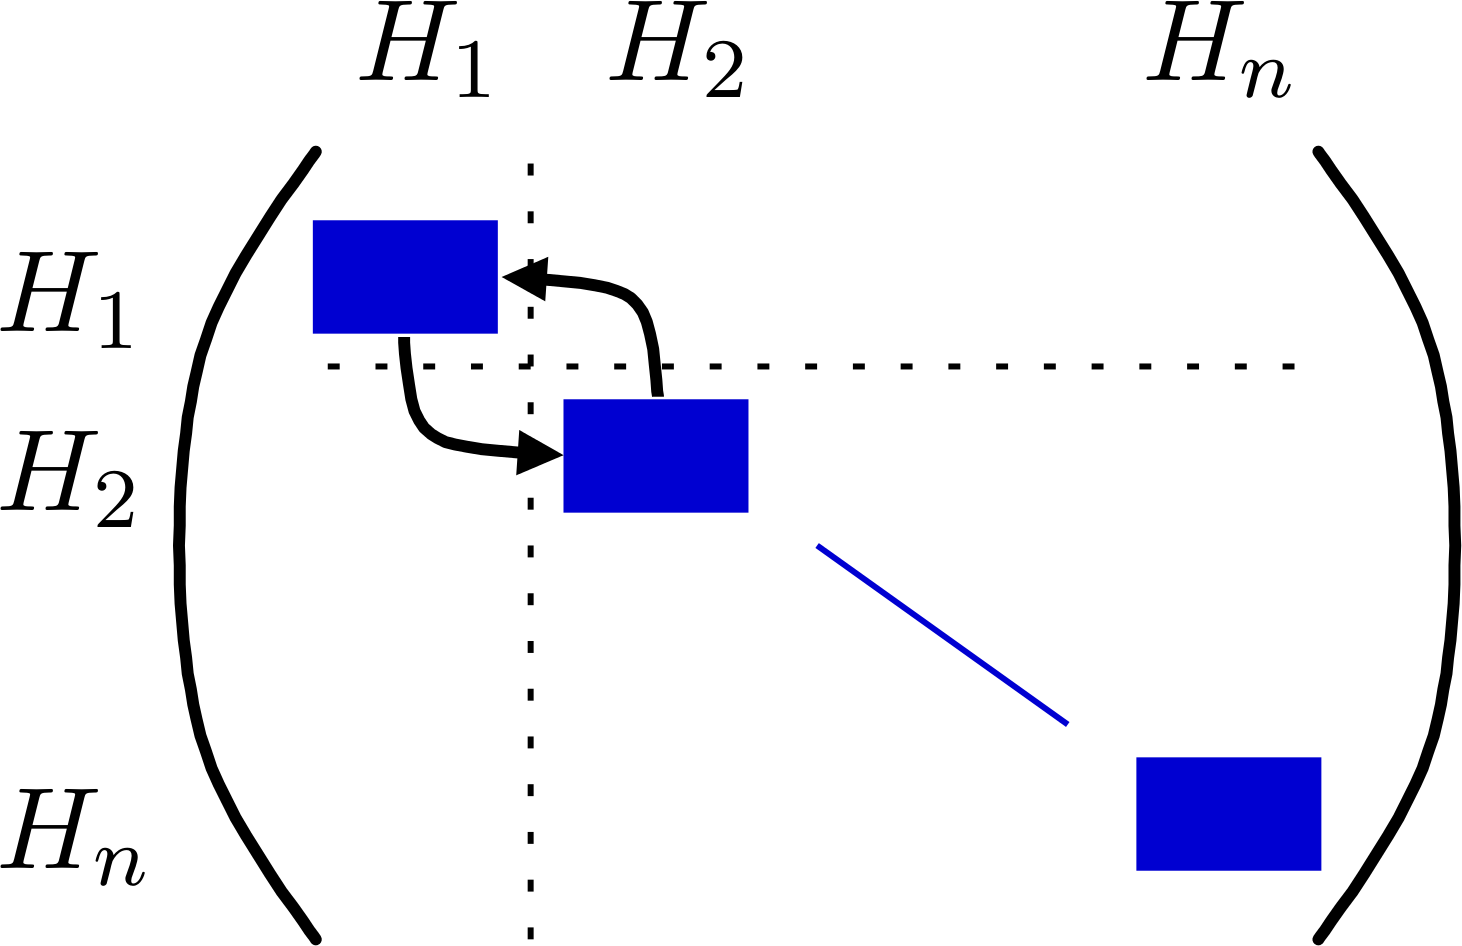
\includegraphics[width=0.45\textwidth]{matrix-structure-2}
  \end{center}
 \end{block}
%  \vspace*{-0.4cm}

\end{frame}




\begin{frame}{Parallelization}
  \vspace{-1.25cm}
  \begin{center}
   Benchmark results for a FinFET (INTEL Core i7 960, NVIDIA GTX 580) \\
   \vspace*{0.5cm}
  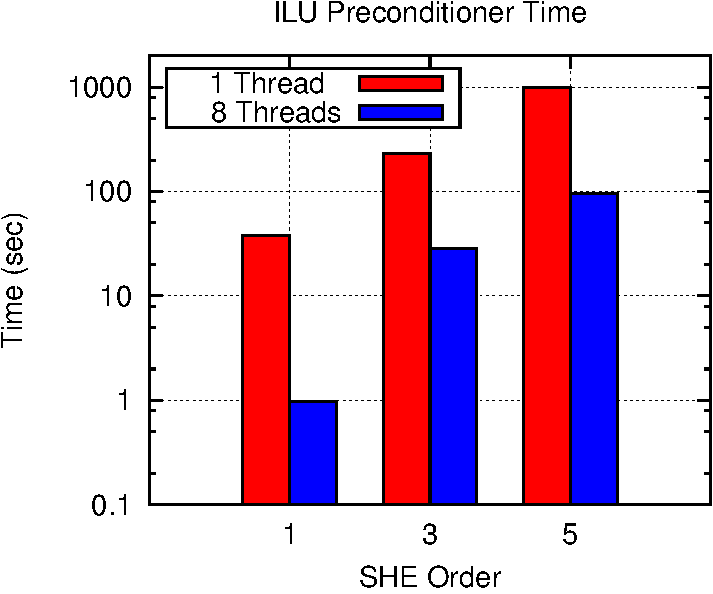
\includegraphics[width=0.48\textwidth]{mosfet-precondtimes} \hspace*{0.2cm}
  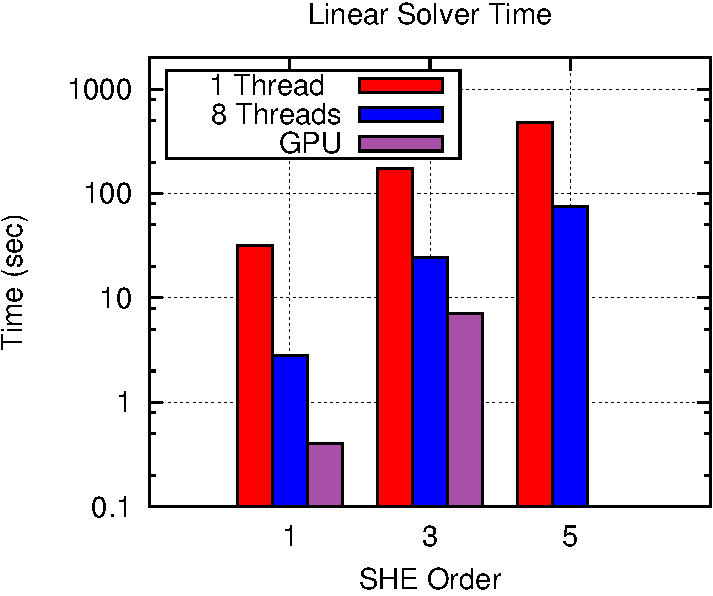
\includegraphics[width=0.48\textwidth]{mosfet-solvertimes}
  \end{center}
\end{frame}

\begin{frame}{Parallelization}
  \begin{center}
   Benchmark results for a FinFET (INTEL Core i7 960, NVIDIA GTX 580) \\
   \vspace*{0.5cm}
   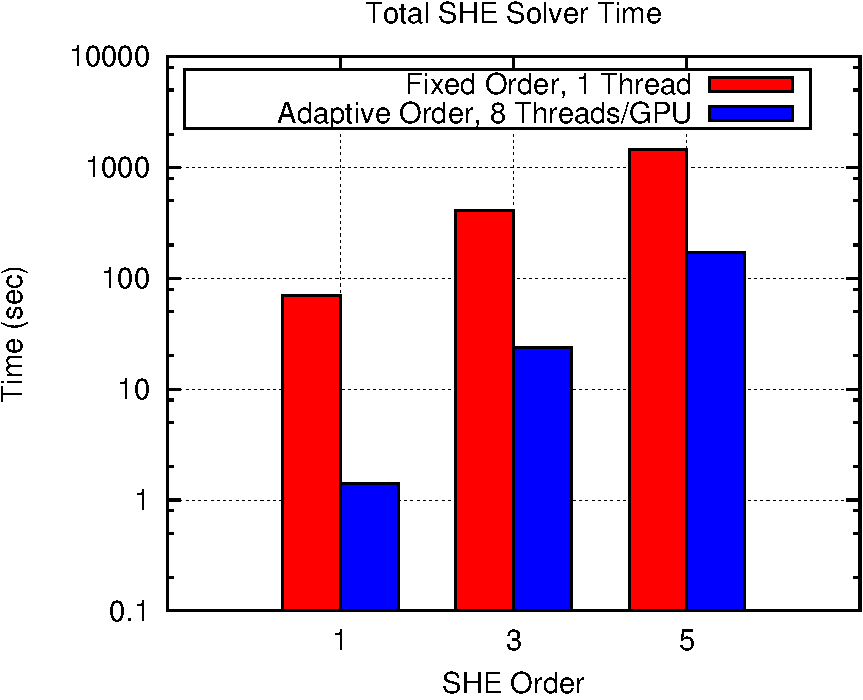
\includegraphics[width=0.7\textwidth]{mosfet-totaltimes}
  \end{center}
\end{frame}



%
% Results
%

\section{Results}


\begin{frame}{Results}
%  \vspace{-0.5cm}
  \begin{minipage}{0.99\textwidth}
   \begin{center}
    Electron Concentration (cm$^{-3}$) \\
    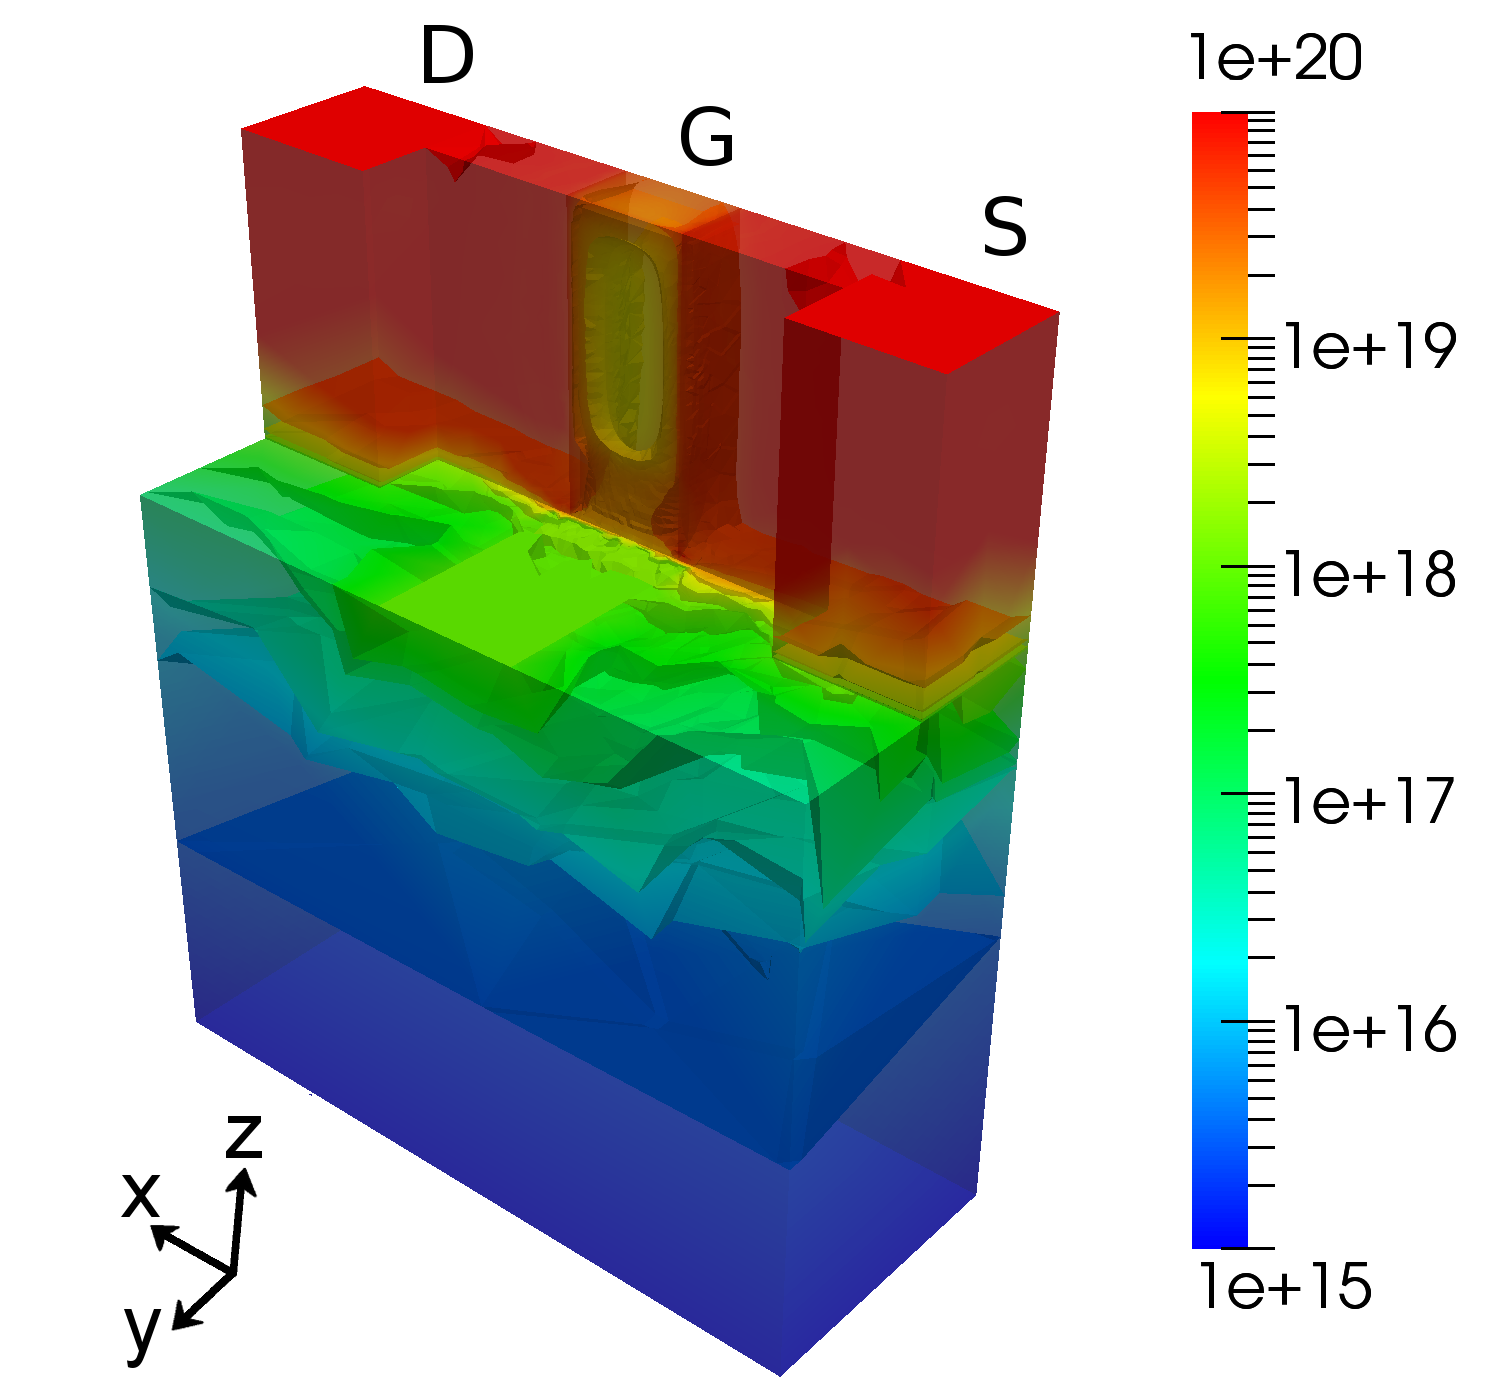
\includegraphics[width=0.31\textwidth]{trigate-n-1} \hspace{1cm}
    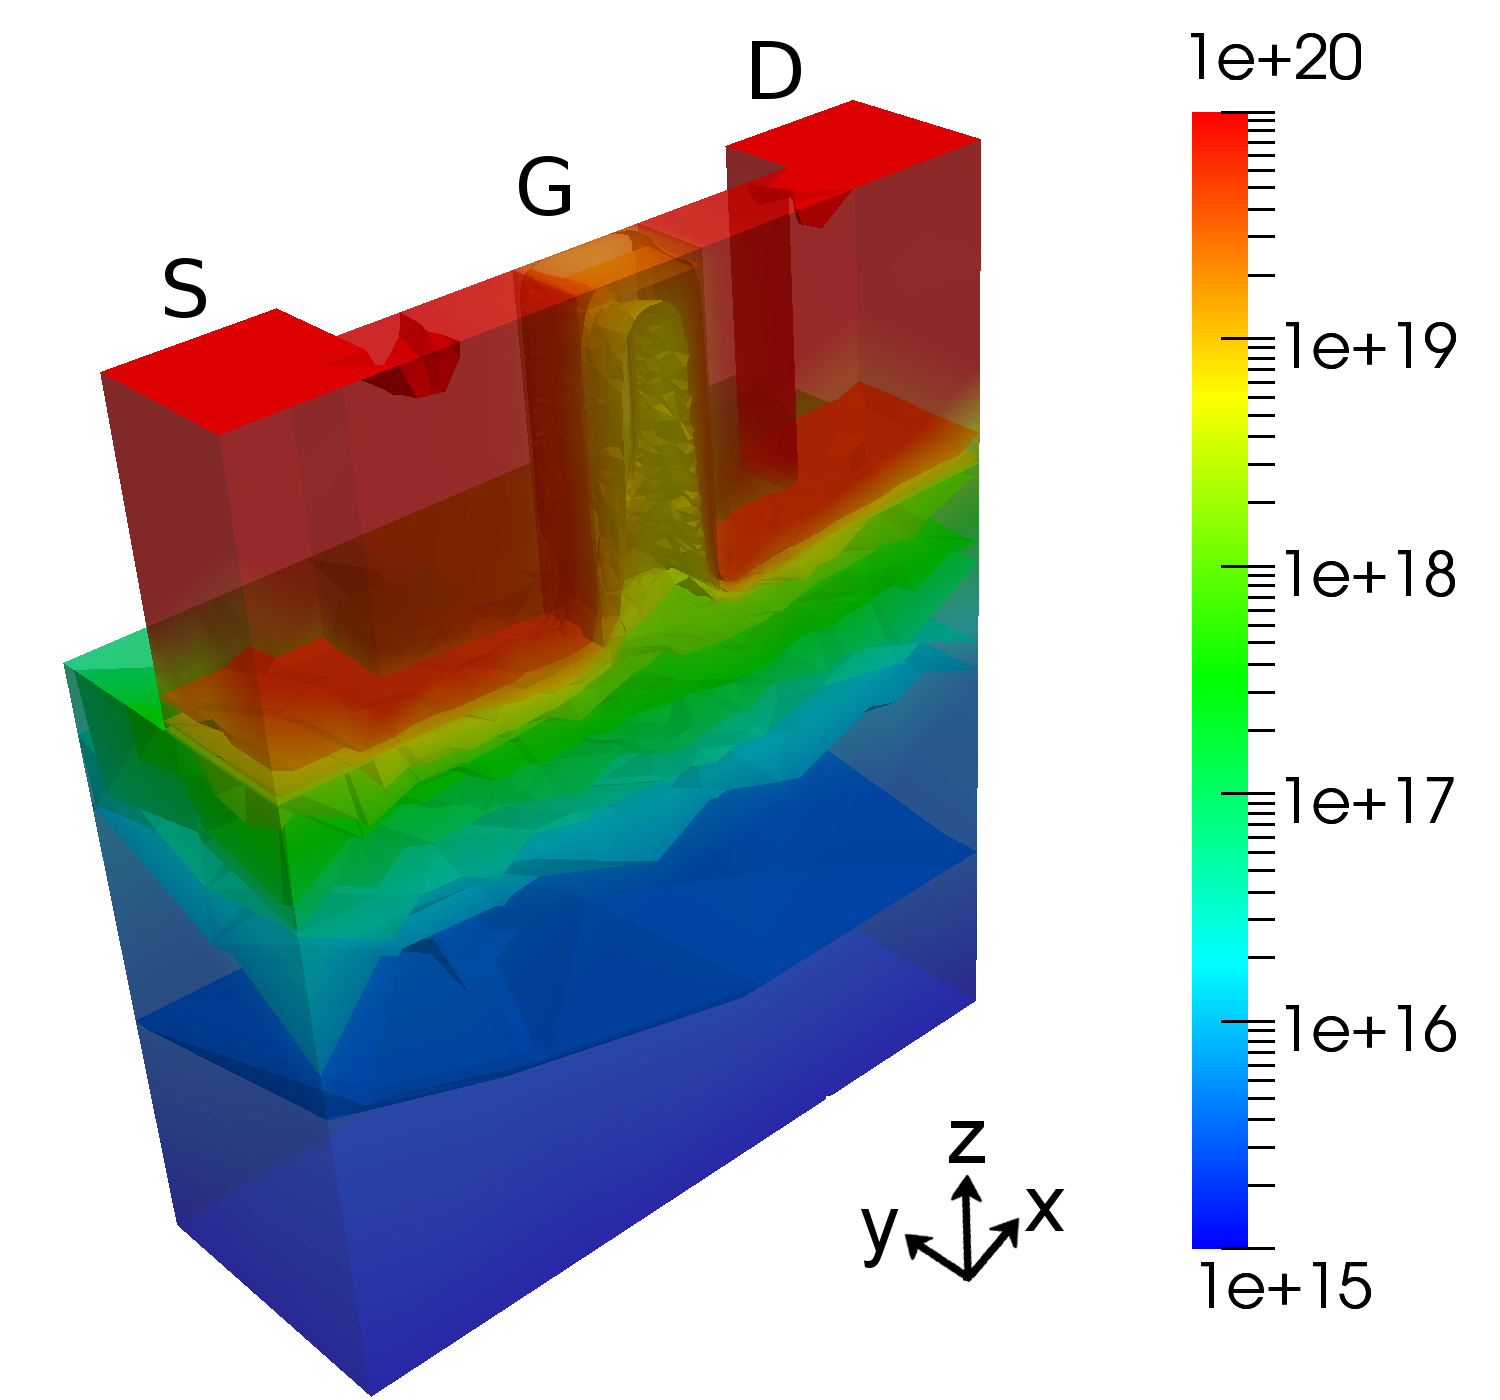
\includegraphics[width=0.31\textwidth]{trigate-n-2}
   \end{center}
  \end{minipage}
    
  \vspace{0.5cm}
  \fcolorbox{white}{white}{
  \begin{minipage}{0.99\textwidth}
   \begin{center}
    Avg.~Expansion Order  \\
    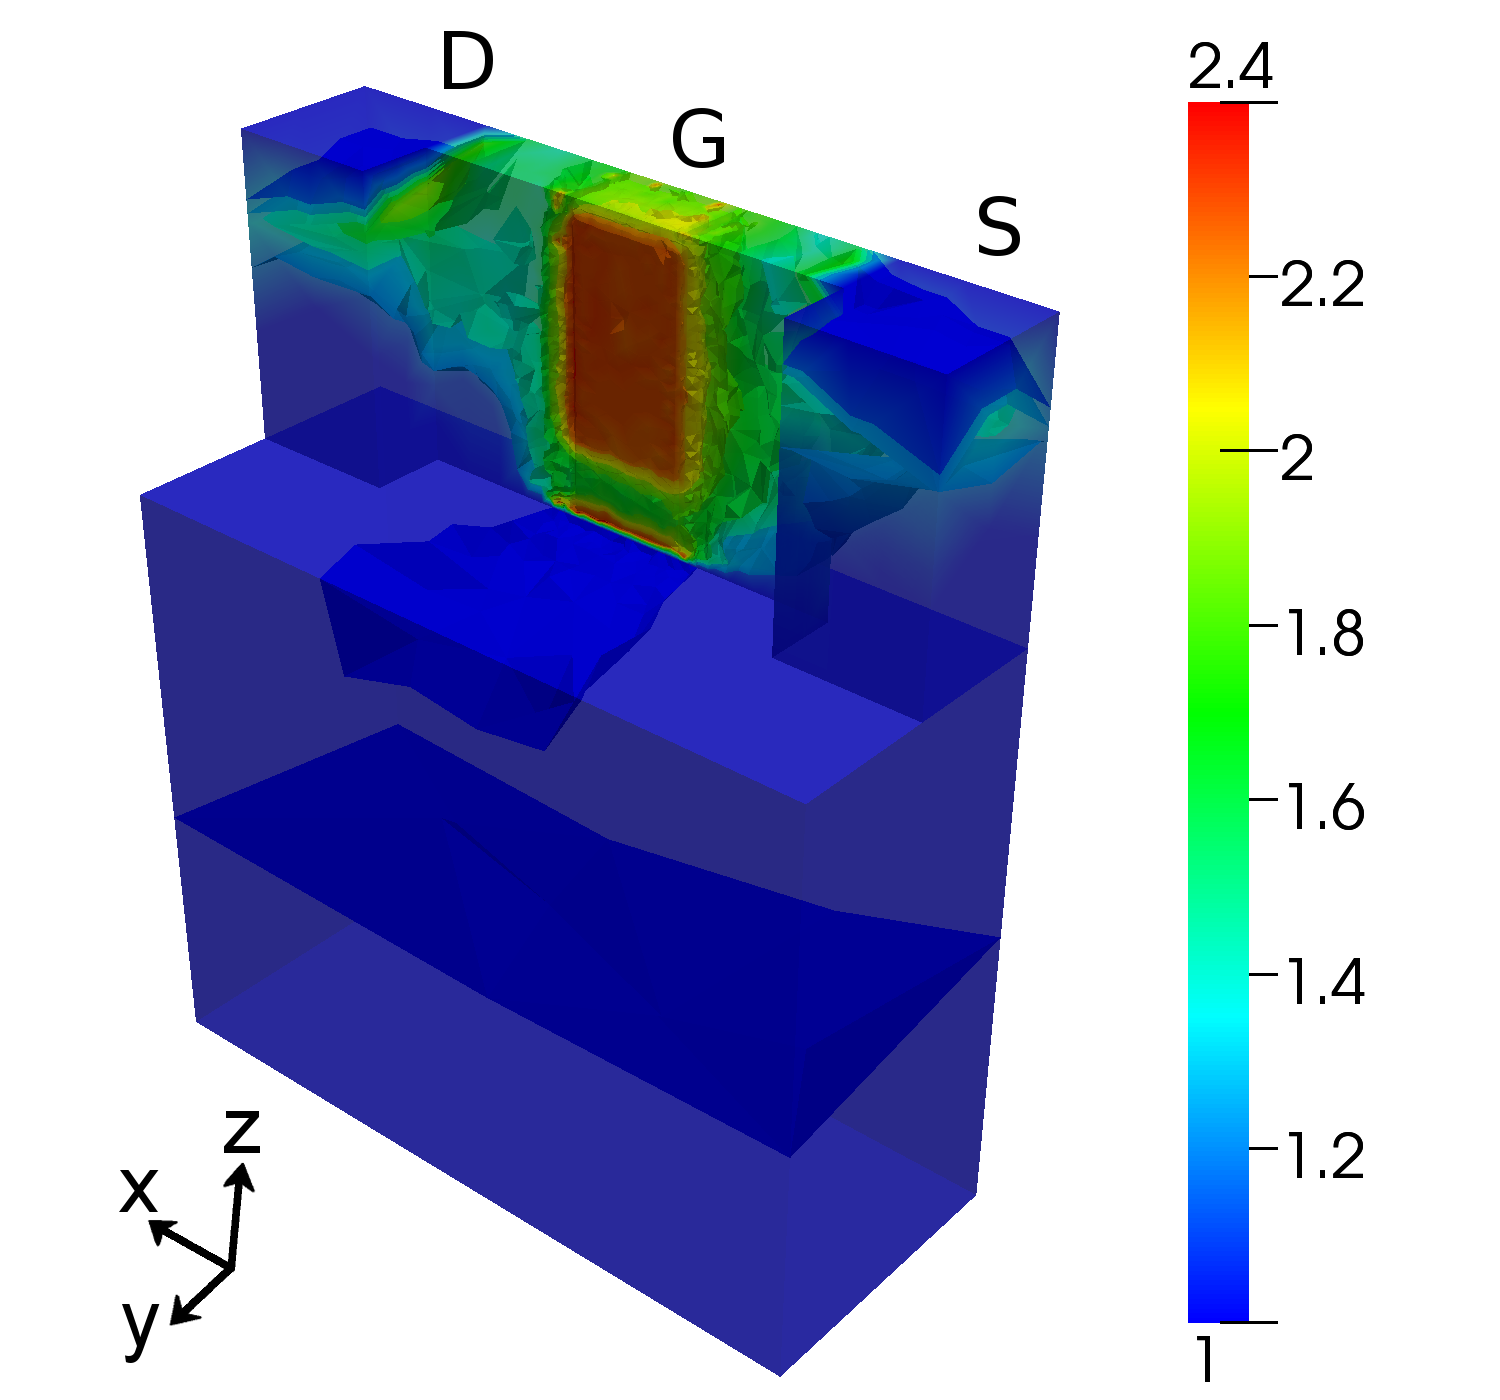
\includegraphics[width=0.31\textwidth]{trigate-avg-order-1} \hspace{1cm}
    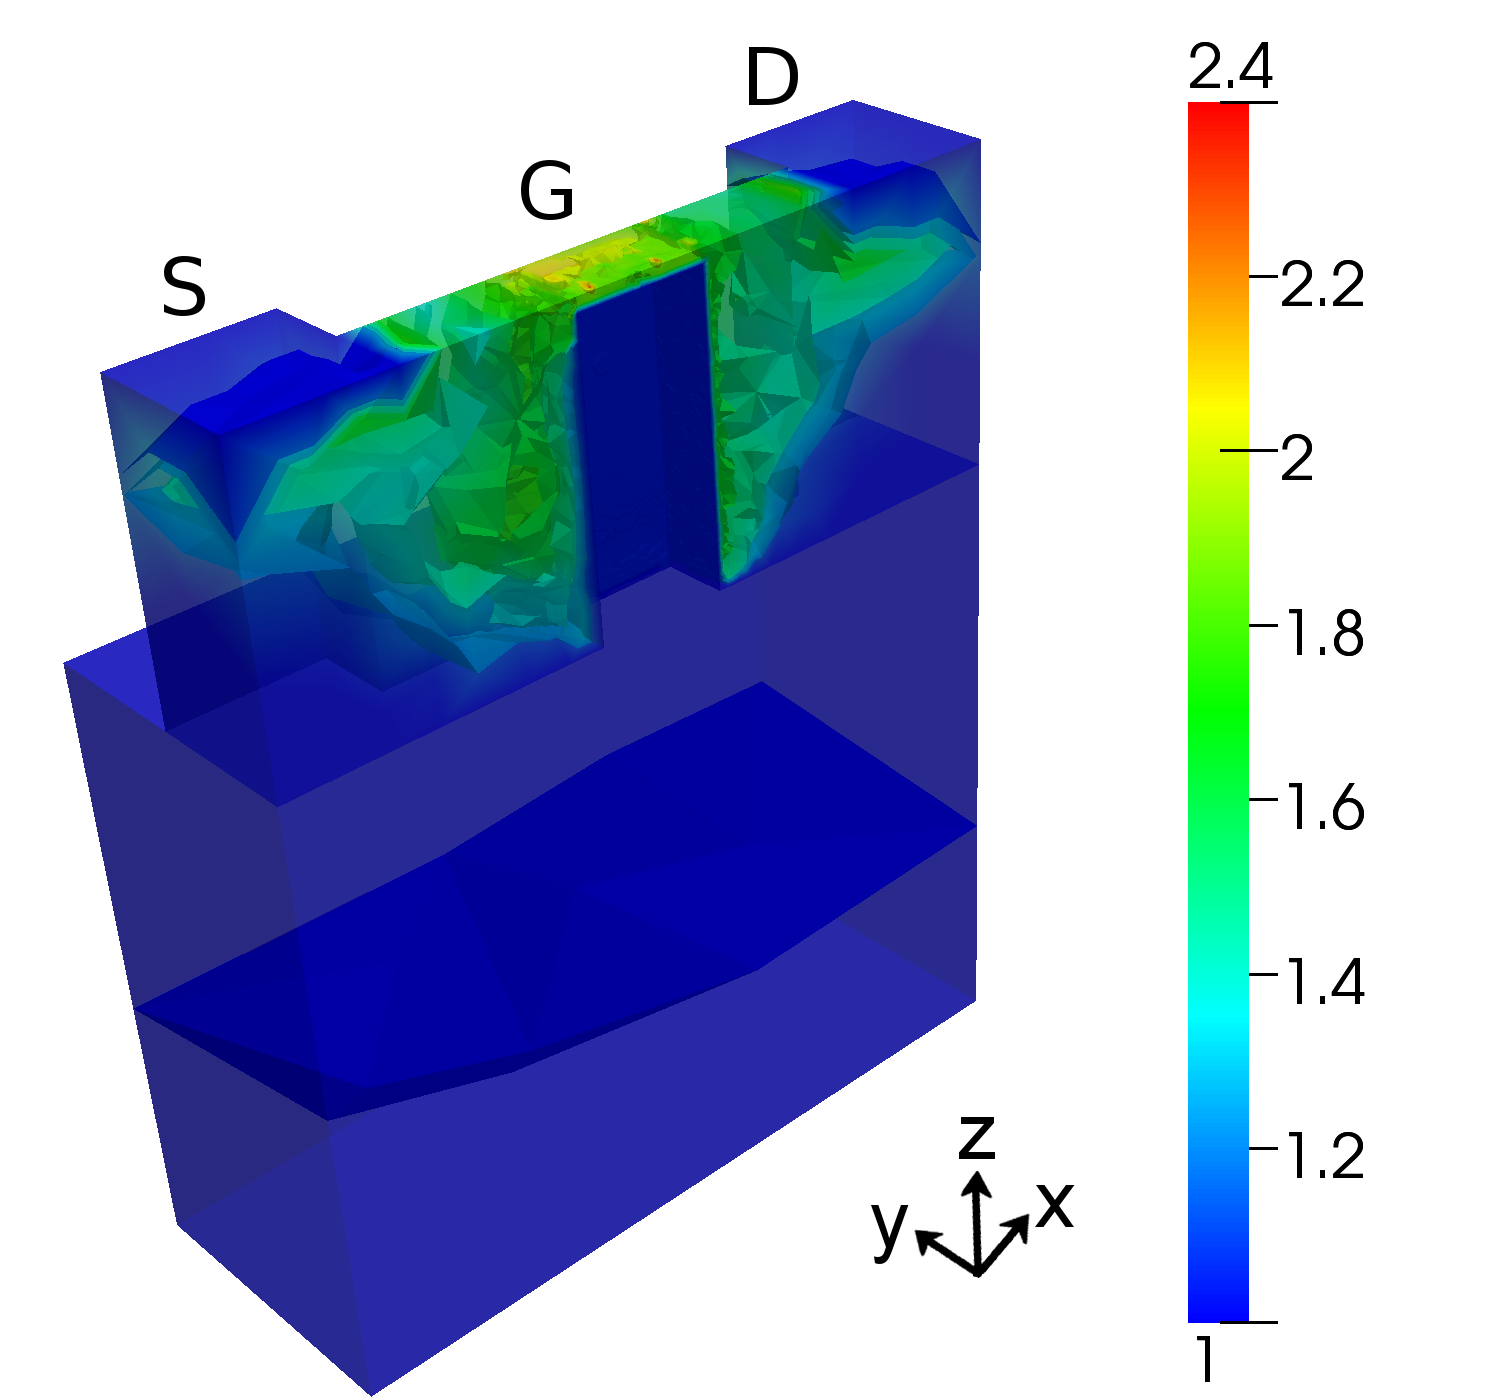
\includegraphics[width=0.31\textwidth]{trigate-avg-order-2}
   \end{center}
  \end{minipage}}
%  \vspace*{-0.5cm}
\end{frame}



\begin{frame}{Results}
%  \vspace{-0.5cm}
  \begin{minipage}{0.99\textwidth}
   \begin{center}
    Electron Concentration (cm$^{-3}$) \\
    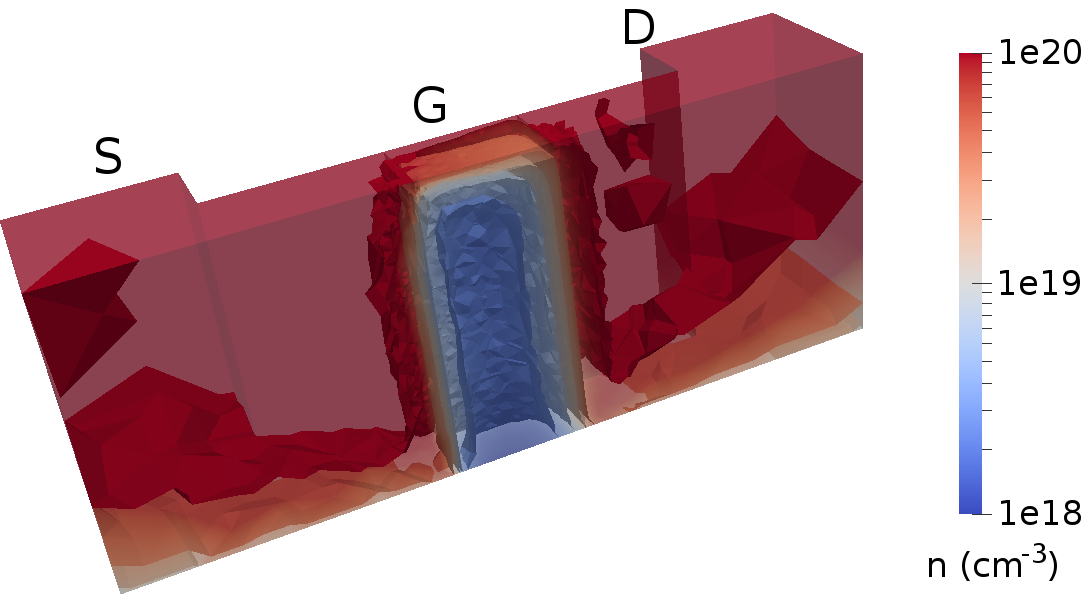
\includegraphics[width=0.51\textwidth]{trigate-electrons-mod}
   \end{center}
  \end{minipage}
    
  \vspace{0.5cm}
  \fcolorbox{white}{white}{
  \begin{minipage}{0.99\textwidth}
   \begin{center}
    Electron Density with Energy above 1eV (cm$^{-3}$)  \\
    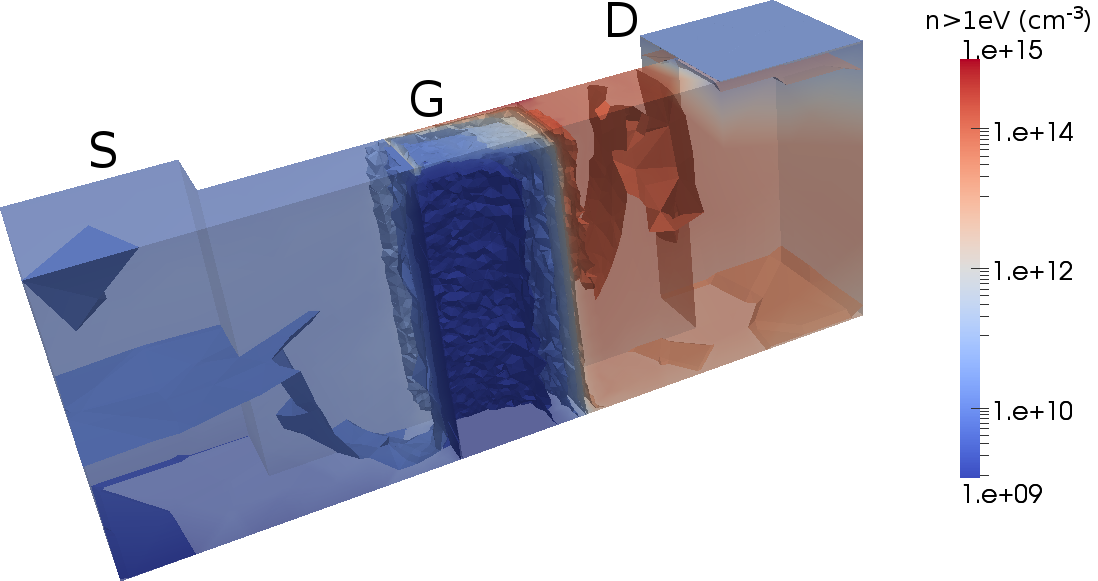
\includegraphics[width=0.51\textwidth]{trigate-electrons1eV-mod.png}
   \end{center}
  \end{minipage}}
%  \vspace*{-0.5cm}
\end{frame}




%
% Summary
%

\section{Summary}

% \begin{frame}{Summary}
%   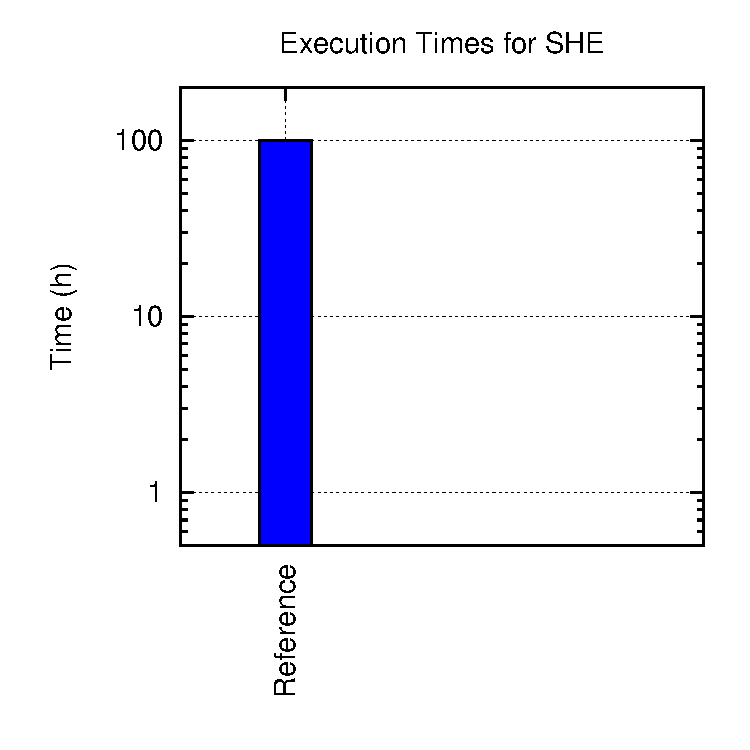
\includegraphics[width=0.49\textwidth]{summary-exec-1}
%   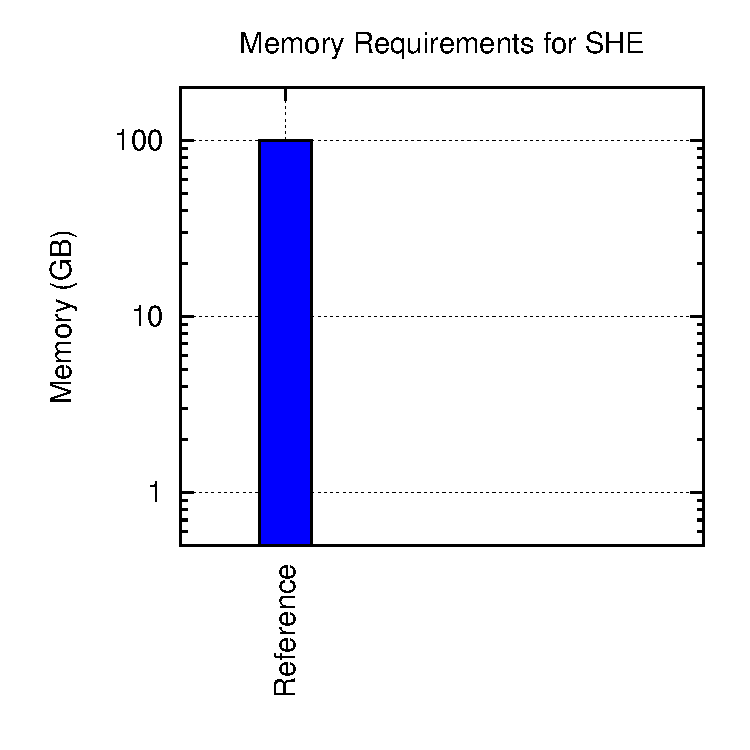
\includegraphics[width=0.49\textwidth]{summary-memory-1}
% \end{frame}
% 
% \begin{frame}{Summary}
%  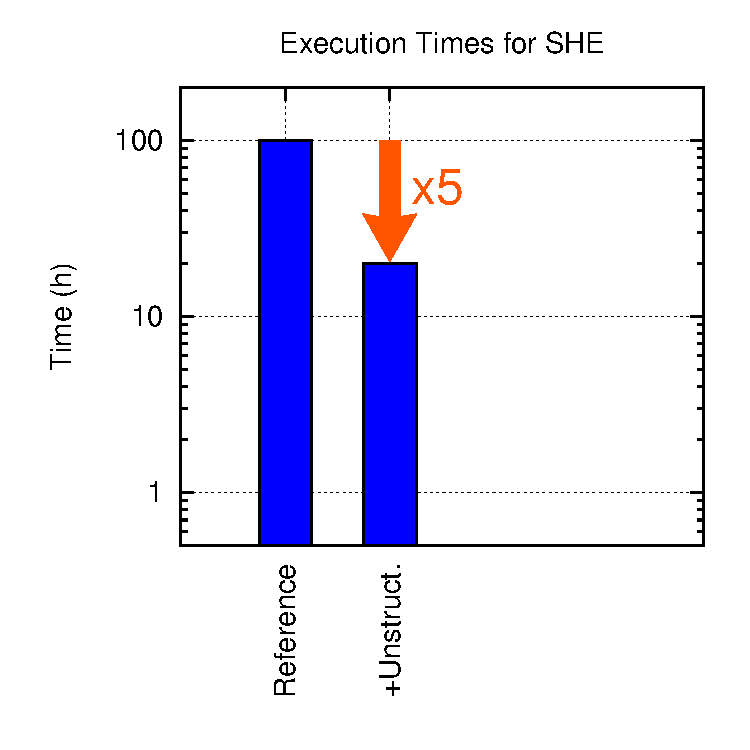
\includegraphics[width=0.49\textwidth]{summary-exec-2}
%  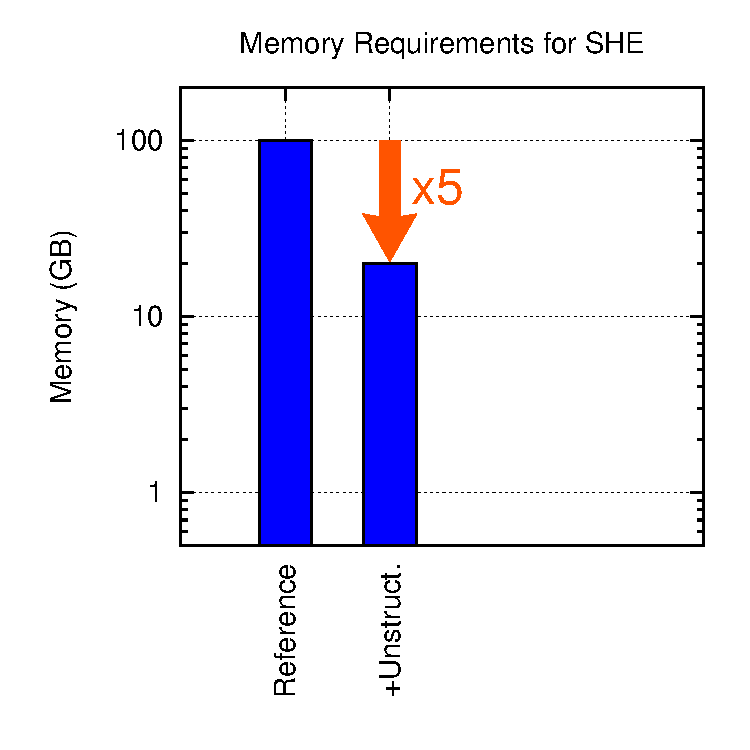
\includegraphics[width=0.49\textwidth]{summary-memory-2}
% \end{frame}
% 
% \begin{frame}{Summary}
%   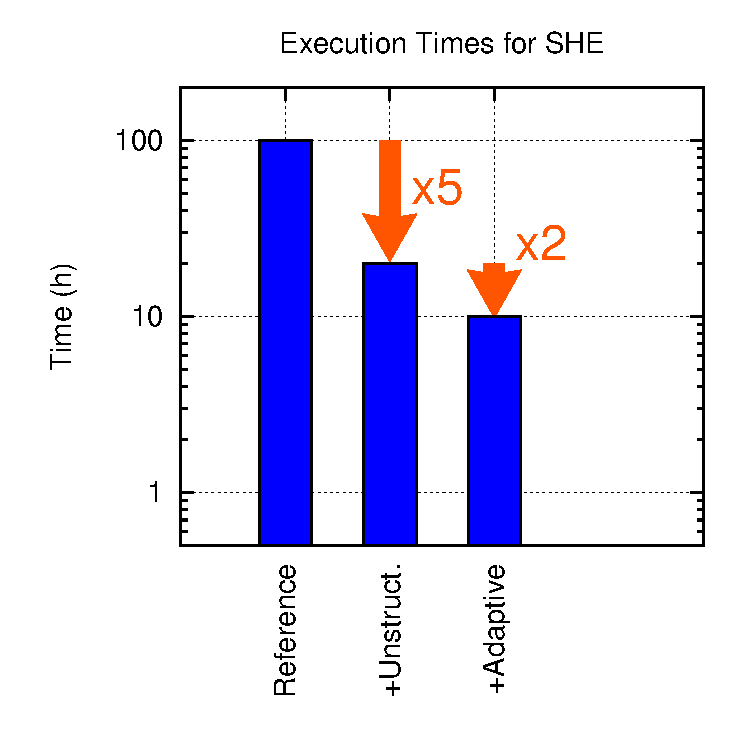
\includegraphics[width=0.49\textwidth]{summary-exec-3}
%   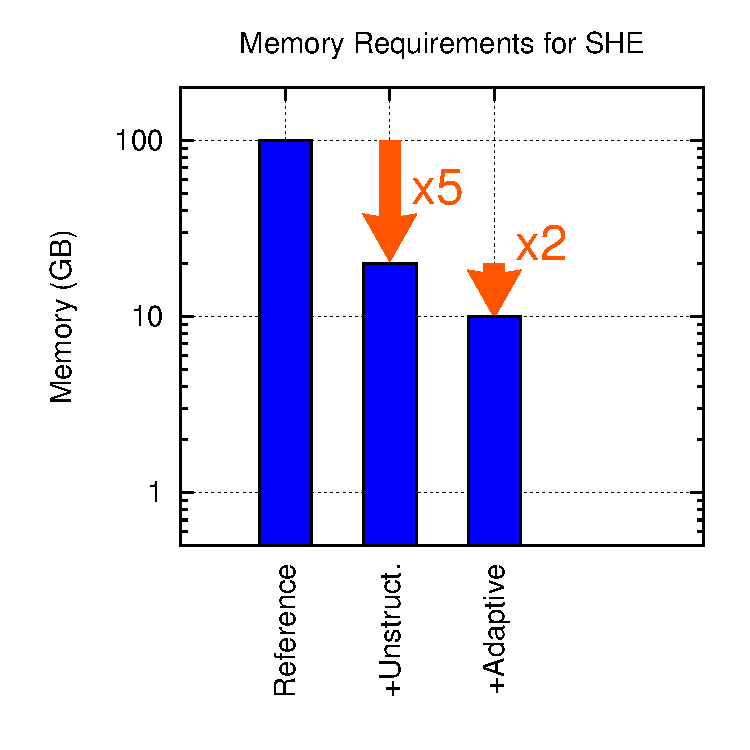
\includegraphics[width=0.49\textwidth]{summary-memory-3}
% \end{frame}

\begin{frame}{Summary}
  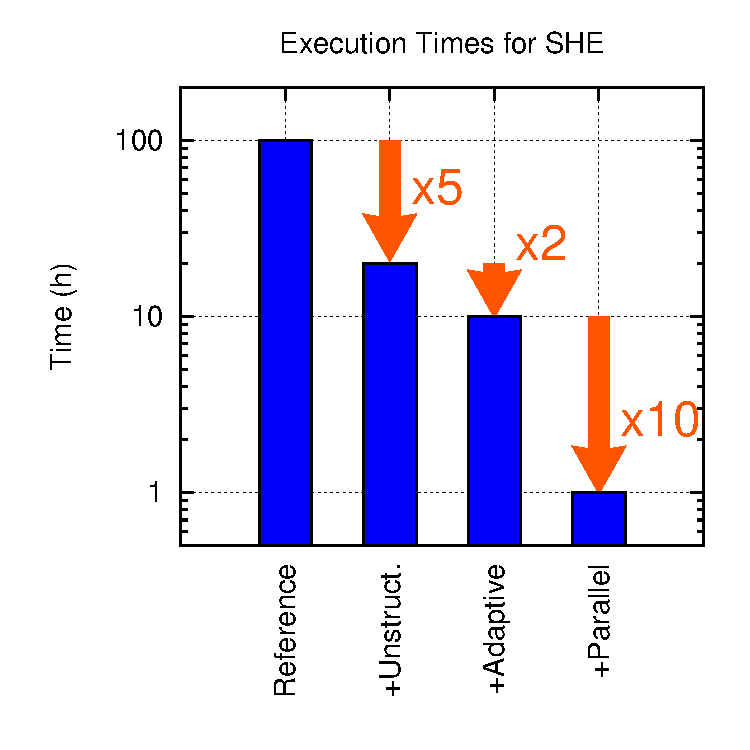
\includegraphics[width=0.49\textwidth]{summary-exec-all}
  \includegraphics[width=0.49\textwidth]{summary-memory-all}
\end{frame}

%%%%%%%%%%% Part 2 %%%%%%%%%%%%%%

\begin{frame}{ViennaSHE}
  \begin{block}{Features}
   \begin{itemize}
    \item Unstructured grids in 1d, 2d, 3d
    \item Adaptive variable-order expansions
    \item Parallelization (shared memory, GPUs)
    \item Carrier-carrier scattering
    \item Free open source MIT/X11 license
   \end{itemize}
  \end{block}
  
  \begin{block}{Rationale}
   \begin{itemize}
    \item Open Science
    \item Reproducibility
    \item Extensibility
    \item ``More than toy problems''
   \end{itemize}
  \end{block}
  
\end{frame}

\begin{frame}{Development Infrastructure}
  \begin{block}{Developer Repository on GitHub}
   \begin{center}
    \includegraphics[width=0.99\textwidth]{figures/viennashe-github}
   \end{center}
  \end{block}
\end{frame}

\begin{frame}{Development Infrastructure}
  \begin{block}{Nightly Test Suite}
   \begin{center}
    \includegraphics[width=0.99\textwidth]{figures/viennashe-nightly}
   \end{center}
  \end{block}
\end{frame}

\begin{frame}{Development Infrastructure}
  \begin{block}{Library Centric Development}
   \begin{center}
    \includegraphics[width=0.94\textwidth]{figures/viennashe-web} \\
    http://viennashe.sourceforge.net/
   \end{center}
  \end{block}
\end{frame}


\begin{frame}{User Requirements}

  \begin{block}{Input/Output}
   \begin{itemize}
    \item Reader/writer for commercial file formats
    \item Material parameter tweaks
    \item Robustness of solver
   \end{itemize}
  \end{block}
  
  \begin{block}{Lessons Learnt}
   \begin{itemize}
    \item C++ is a golden cage
    \item Long-term investments in research hard
    \item Each parameter needs to adjustable
   \end{itemize}
  \end{block}
  
\end{frame}


\begin{frame}{Conclusion}

  \begin{block}{SHE Method}
   \begin{itemize}
    \item Viable alternative to Monte Carlo
    \item Full 3d device simulations possible
    \item Convergence behavior similar to drift-diffusion model
   \end{itemize}
  \end{block}
  
  %\pause
  
  \begin{block}{ViennaSHE}
   \begin{itemize}
    \item Free open source simulator based on SHE method
    \item Fully open development infrastructure
    \item http://viennashe.sourceforge.net/
   \end{itemize}
  \end{block}
  
  %\pause
  
  \begin{center}
   \Large \textbf{Thanks to the organizers for AMaSiS 2015!}
  \end{center}

  
\end{frame}


\end{document}

